\section{MeROS metamodel}
\label{sec:metamodel}

MeROS metamodel is formulated according to the requirements discussed in the previous section. Sec.~\ref{sec:metamodel-composition} presents MeROS blocks' structural composition, and sec.~\ref{sec:metamodel-communication} describes inter-component communication. From the metamodel perspective, the structural aspects [R2] are formulated in both sections, while behavioural [R1] is in the latter. The diagrams comprise selected requirements being allocated to expose the MeROS metamodel development process.

The MeROS diagrams were created in the Enterprise Architect development tool within the SysML project [R8] and organised in three packages [R6.1] (Fig.~\ref{fig:meros_project_packages_pkg}): (i) Requirement Model related to requirements formulation and analysis, (ii) MeROS -- the metamodel itself, (iii) Rico Controller -- the exemplary ROS~1 application of MeROS described in sec.~\ref{sec:application-example}. The stereotypes are introduced in MeROS metamodel with the dedicated MeROS profile [R6.2].


\begin{figure}[H]
    \centering
    \begin{center}
    {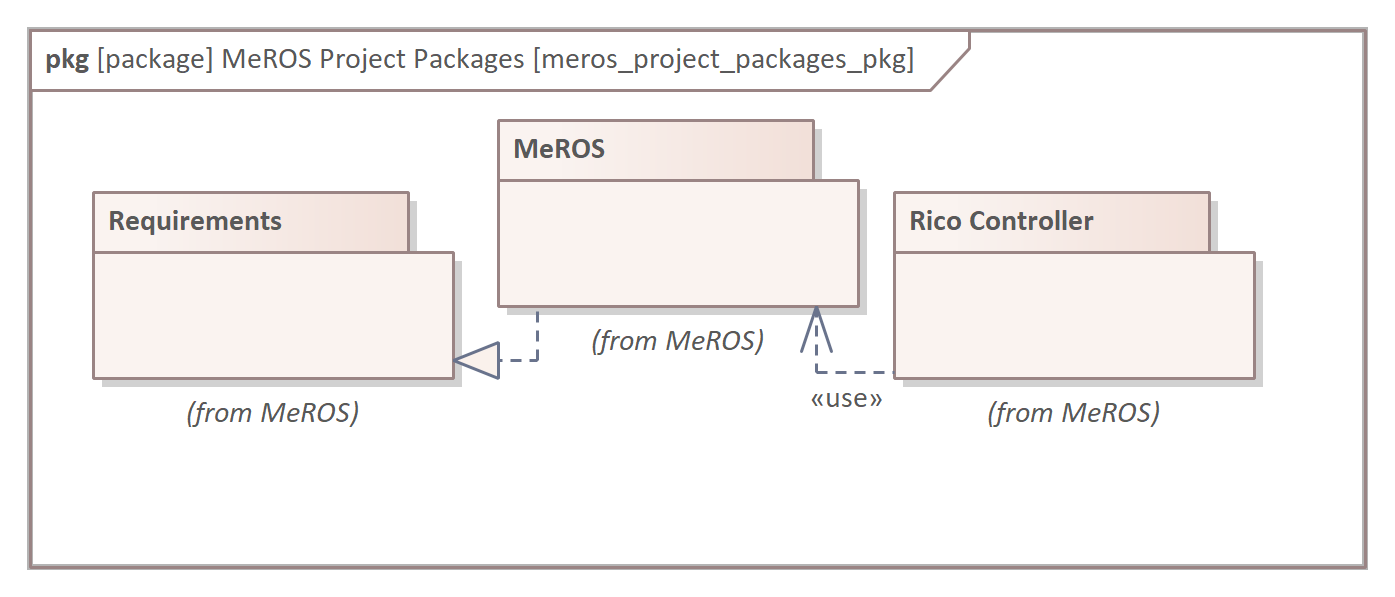
\includegraphics[scale=1.0]{../imgs/meros_project_packages_pkg.png}}
    \end{center}
    \caption{MeROS project SysML packages, where Rico Controller is an exemplary realisation of MeROS metamodel.}
    \label{fig:meros_project_packages_pkg}
\end{figure}

\subsection{Metamodel composition}
\label{sec:metamodel-composition}

The degree of specificity of a metamodel is a compromise between its comprehensiveness (and, therefore, more general formulation) and a more accurate representation of a particular subclass of specific implementations. The metamodel contains compositions of elements and other primary relationships. Attributes and operations range widely, in particular between ROS~1 and ROS~2. Hence, their inclusion would lead to overgrowth and complication of the metamodel [R6]. Models derived from the metamodel can define their operations and new relations specific to a particular system.

The SysML blocks reflect ROS concepts [R3], and their composition is depicted in bdd (block definition diagrams). The metamodel is formulated in a~single SysML package. Hence, Groups of Packages (especially Workspaces) and Intrasystems are composed into ROS System (Fig.~\ref{fig:ros_system_bdd}).


\begin{figure}[H]
    \centering
    \begin{center}
    {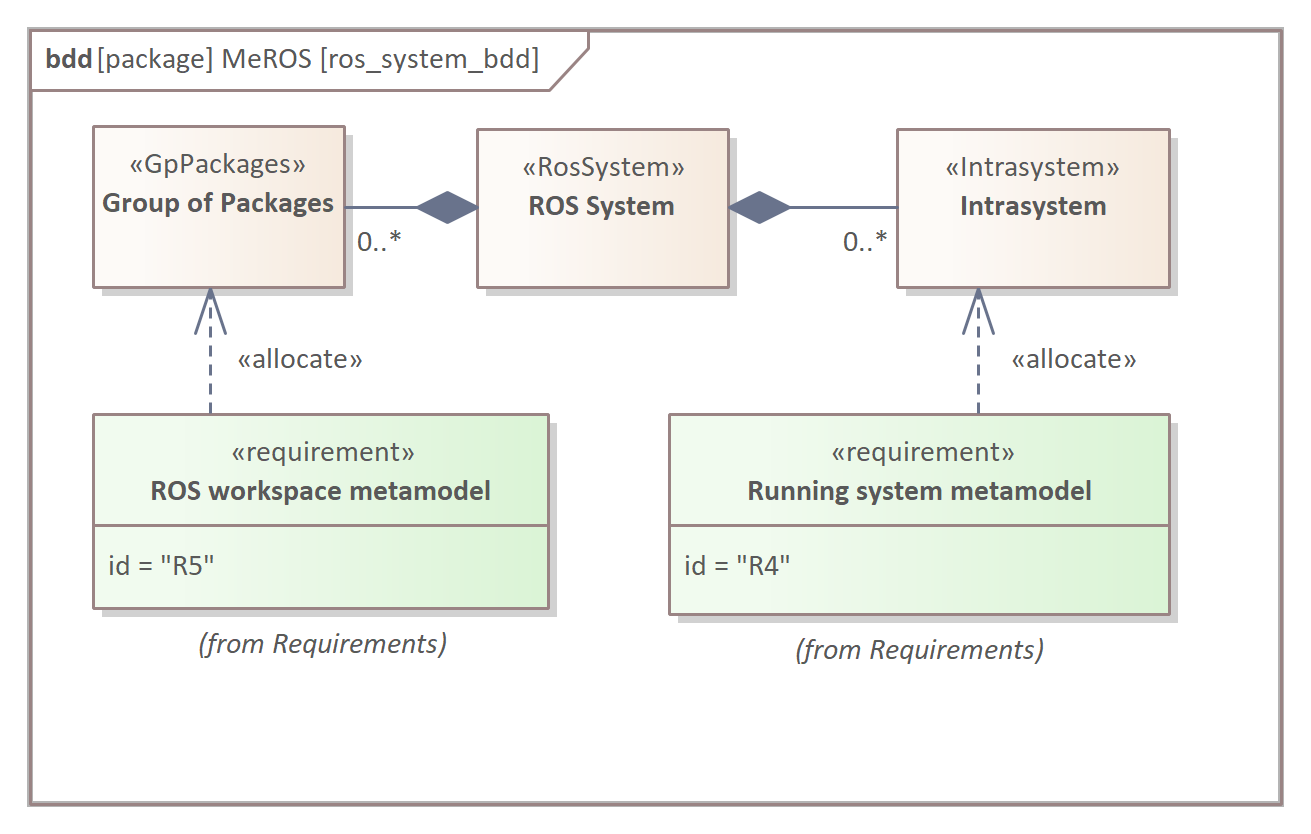
\includegraphics[scale=1.1]{../imgs/meros_pkg/ros_system_bdd.png}}
    \end{center}
    \caption{ROS system general composition -- bdd.}
    \label{fig:ros_system_bdd}
\end{figure}

Consequently, some concepts (e.g., Node) occur in Workspaces and Intrasystems. It reduces the number of SysML blocks in the metamodel [R6.4] and eliminates the need for unnecessary mapping of SysML blocks [R6.5].

\pagebreak

In MeROS, a~Communicating Component (Fig.~\ref{fig:communicating_components_bdd}) is a~crucial abstraction of a~number of ROS concepts to represent their standardised role regarding communication.


\begin{figure}[H]
    \centering
    \begin{center}
    {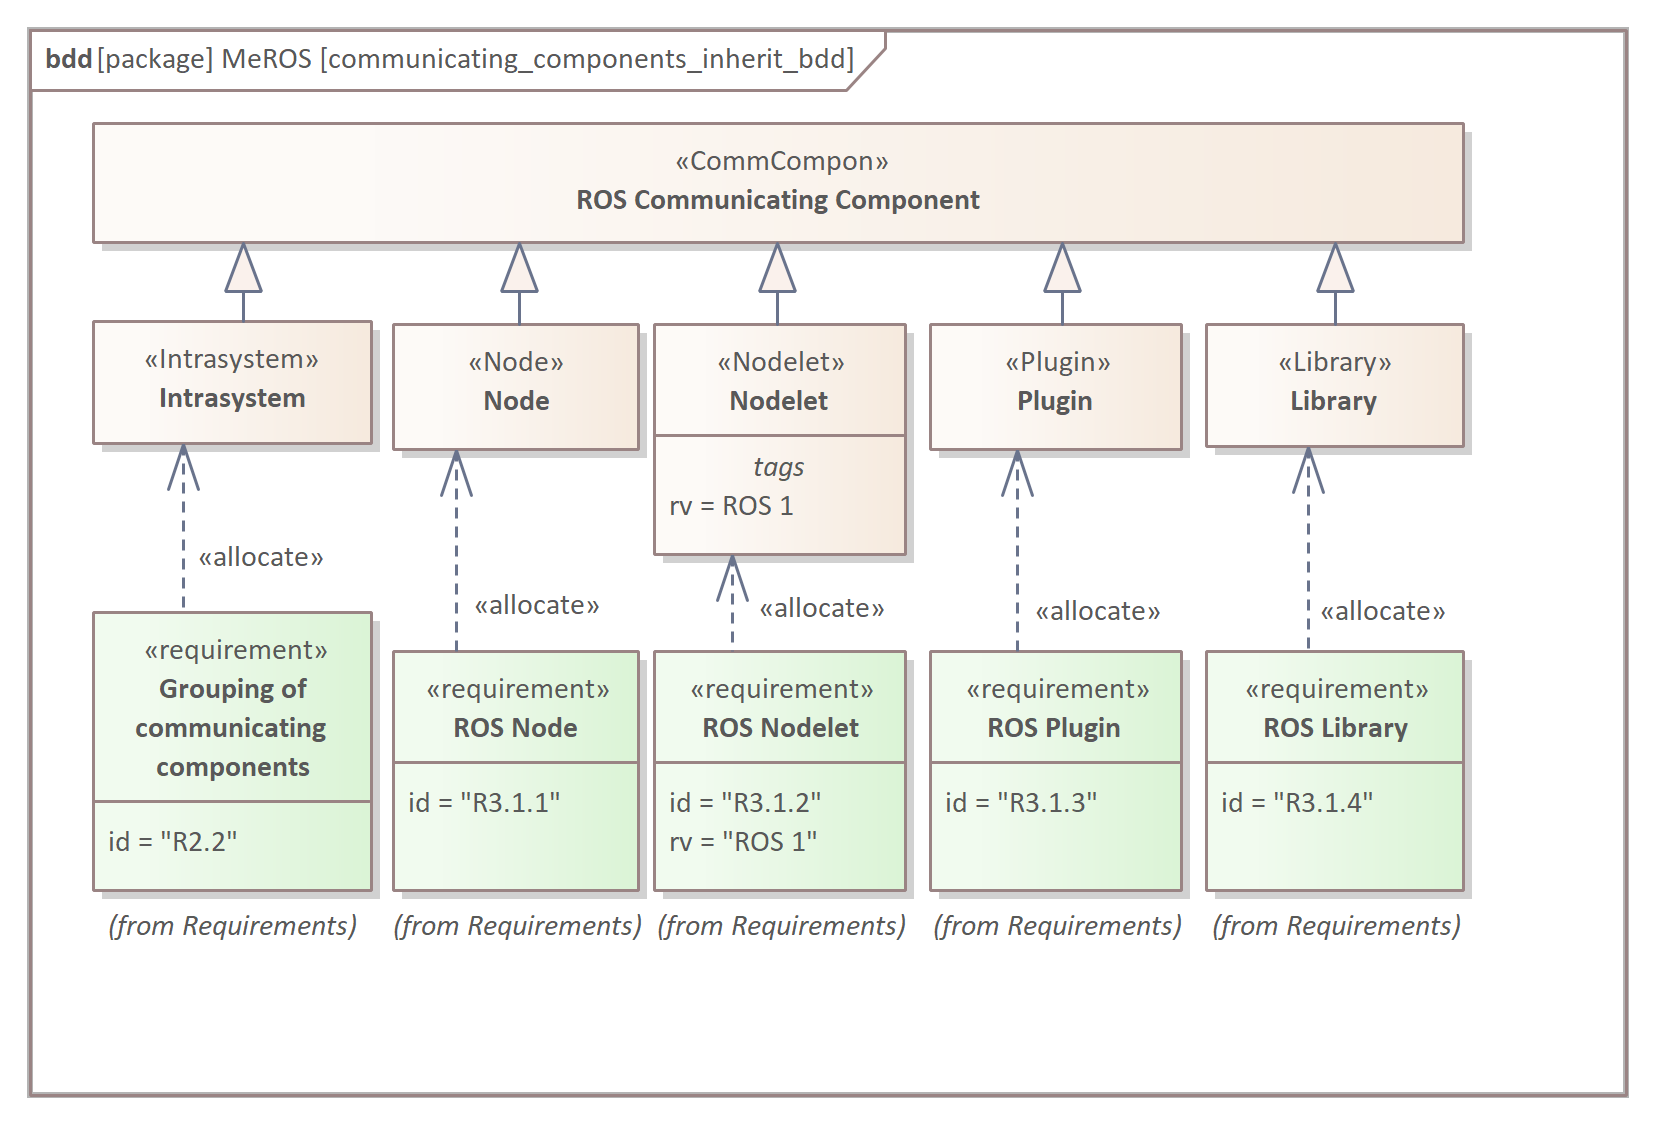
\includegraphics[scale=1]{../imgs/meros_pkg/communicating_components_inherit_bdd.png}}
    \end{center}
    \caption{Communicating Component and specialised blocks -- bdd.}
    \label{fig:communicating_components_bdd}
\end{figure}

It should be noted that behavioural aspects of a~particular model specified in MeROS can be formulated by operation specification as an act (activity), sd (sequence), or stm (state machine) diagrams. The Intrasystem is one of the aggregates added to the base ROS concepts in MeROS.

\pagebreak

For clarity, relations of Communicating Components are depicted in several diagrams. Fig.~\ref{fig:communicating_component_topics_bdd} considers Topics and their Data Structures. Here, the Communicating Component can act as a publisher or a subscriber.


\begin{figure}[H]
    \centering
    \begin{center}
    {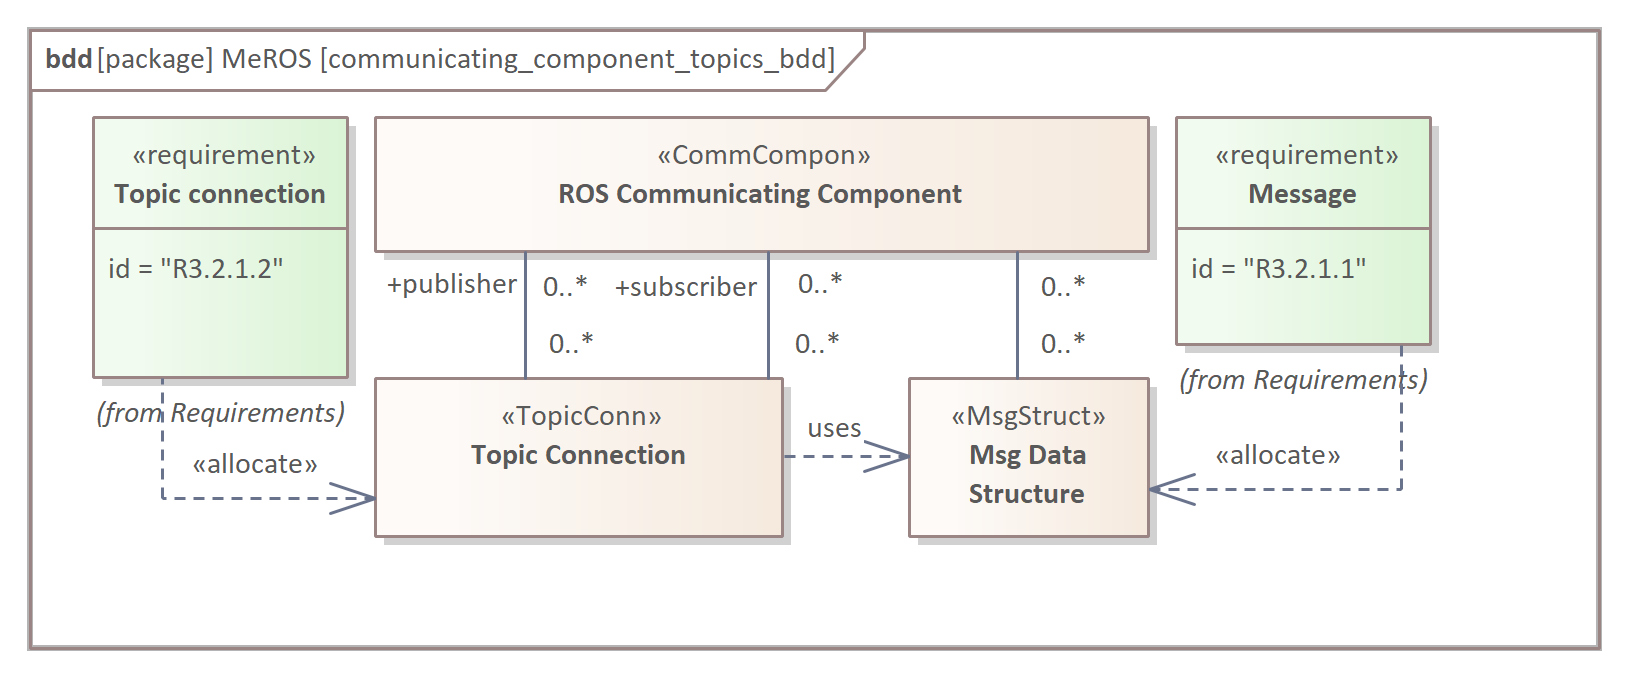
\includegraphics[scale=1.1]{../imgs/meros_pkg/communicating_component_topics_bdd.png}}
    \end{center}
    \caption{Communicating Component relations -- topics -- bdd.}
    \label{fig:communicating_component_topics_bdd}
\end{figure}

Fig.~\ref{fig:communication_blocks_services_bdd} depicts Services and their Data Structures. In this case, the Communicating Component can act as a server or a client.


\begin{figure}[H]
    \centering
    \begin{center}
    {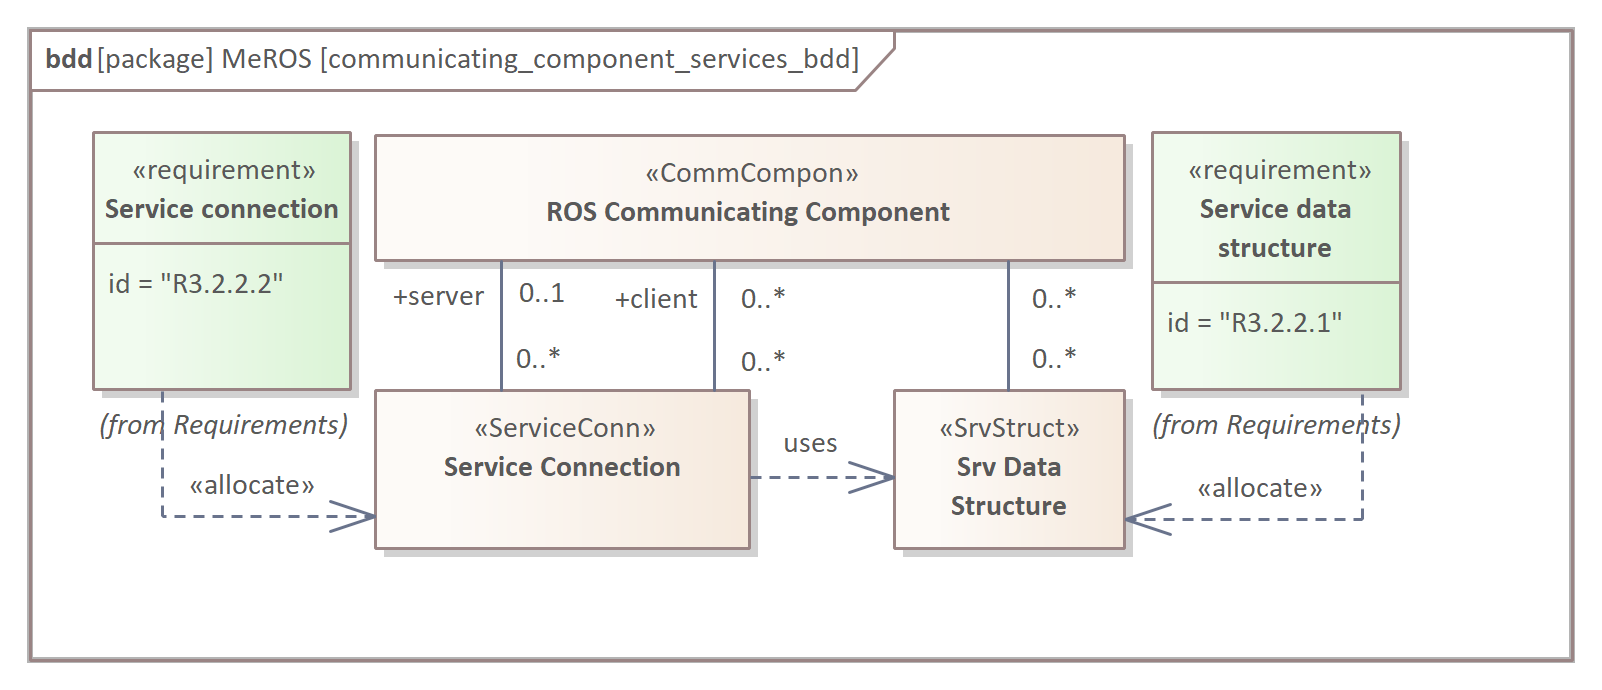
\includegraphics[scale=1.1]{../imgs/meros_pkg/communicating_component_services_bdd.png}}
    \end{center}
    \caption{Communicating Component relations -- services -- bdd.}
    \label{fig:communication_blocks_services_bdd}
\end{figure}
S
In ROS~2, an Action bases on Topics and Services while in ROS~1 only on Topics. From functional point of view, ROS~1 specific Topics included in Action have their equivalents in ROS~2 specific Services.

\pagebreak

The Actions are depicted in two diagrams -- Fig.~\ref{fig:communicating_component_actions_bdd} and Fig.~\ref{fig:action_bdd}. Similarly to Services, the Communicating Component can act as a server or a client.


\begin{figure}[H]
    \centering
    \begin{center}
    {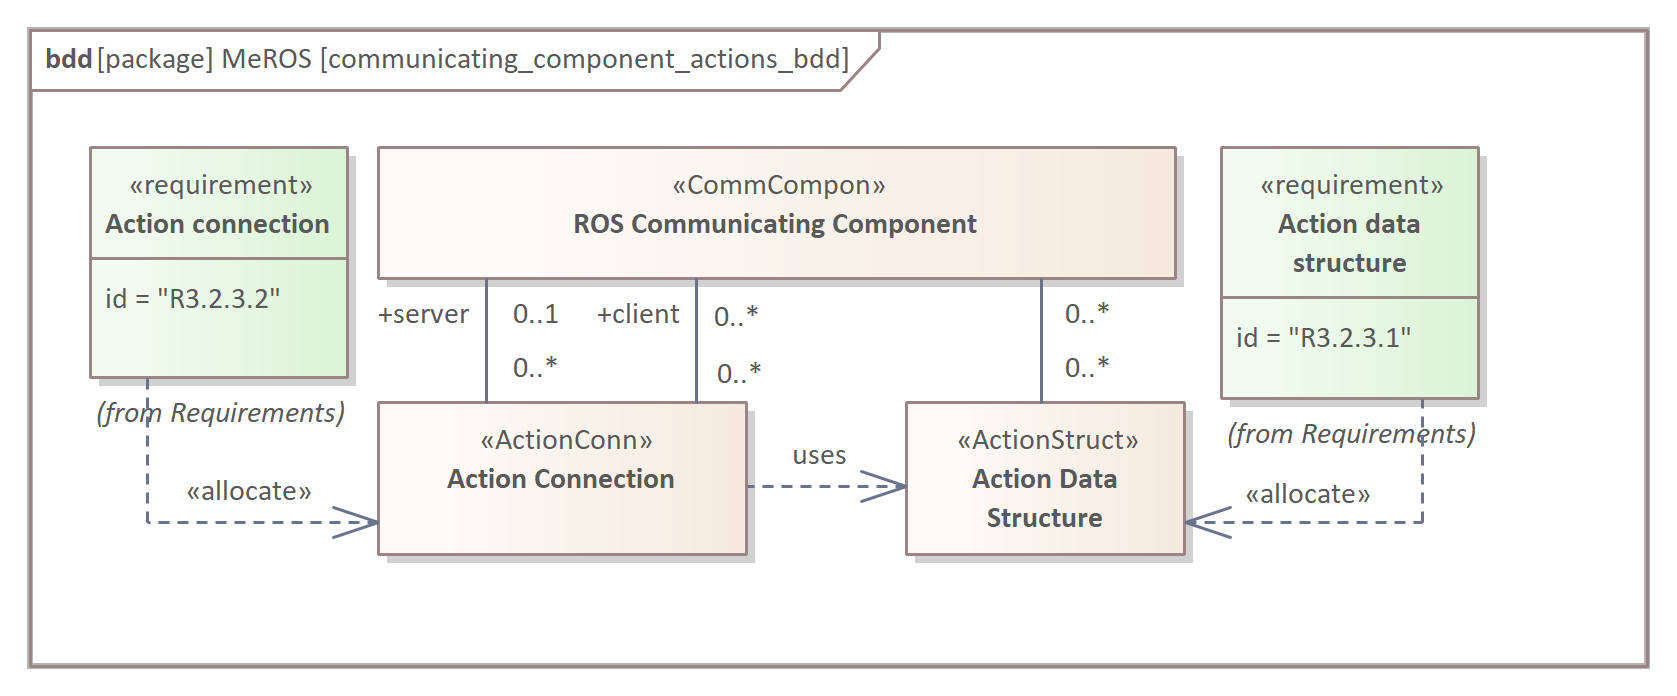
\includegraphics[scale=1]{../imgs/meros_pkg/communicating_component_actions_bdd.png}}
    \end{center}
    \caption{Communicating Component relations -- actions -- bdd.}
    \label{fig:communicating_component_actions_bdd}
\end{figure}

\begin{figure}[hbt]
    \centering
    \begin{center}
    {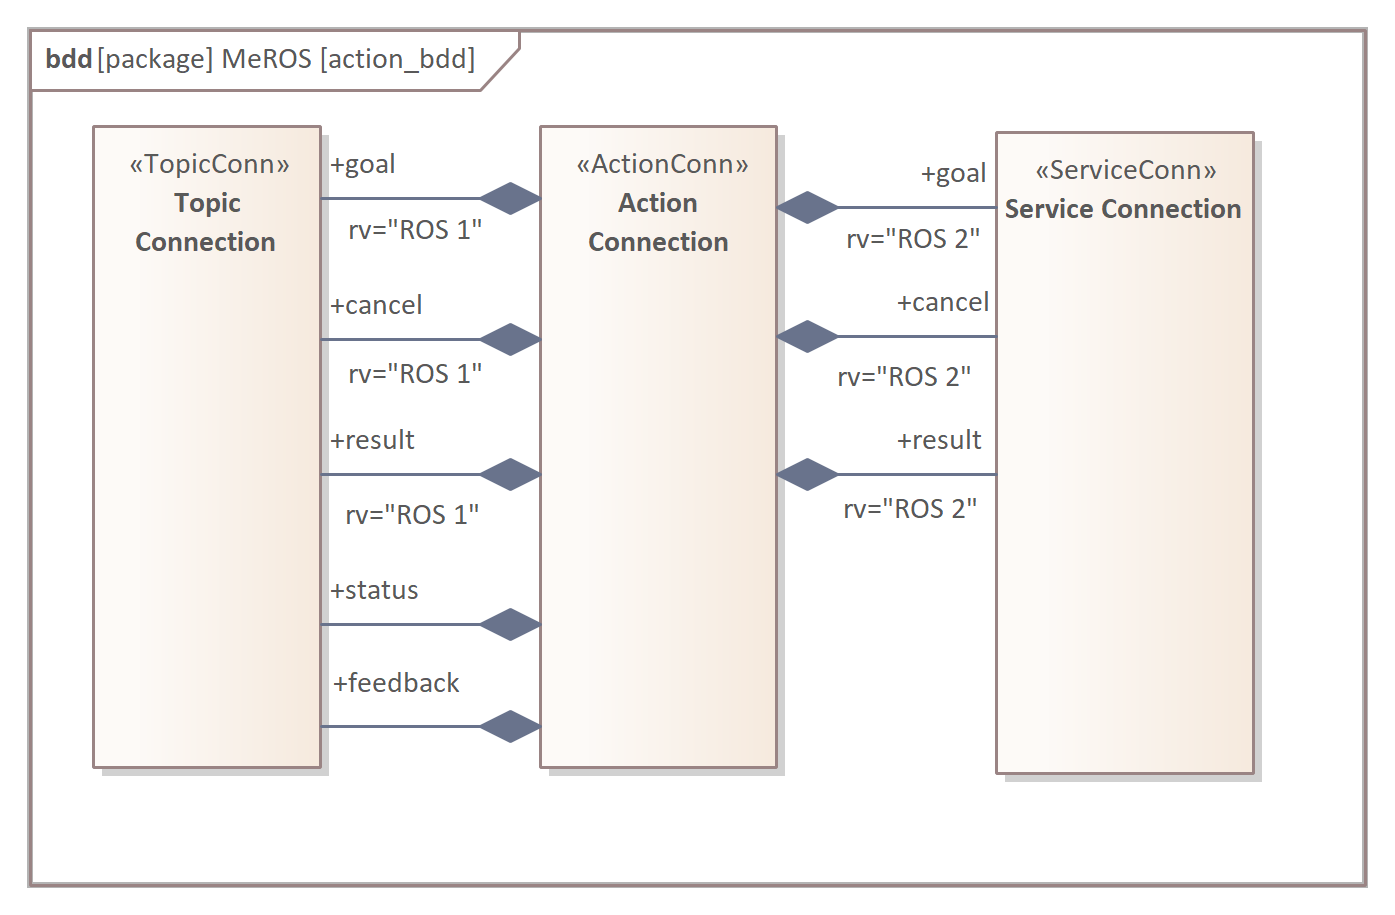
\includegraphics[scale=1.1]{../imgs/meros_pkg/action_bdd.png}}
    \end{center}
    \caption{Action -- bdd.}
    \label{fig:action_bdd}
\end{figure}

\pagebreak

Fig.~\ref{fig:communicating_component_other_bdd} describes how Non-ROS elements are taken into account in relation to communication. Additionally, the figure presents Communication Channel relation to ROS Communicating Component.


\begin{figure}[H]
    \centering
    \begin{center}
    {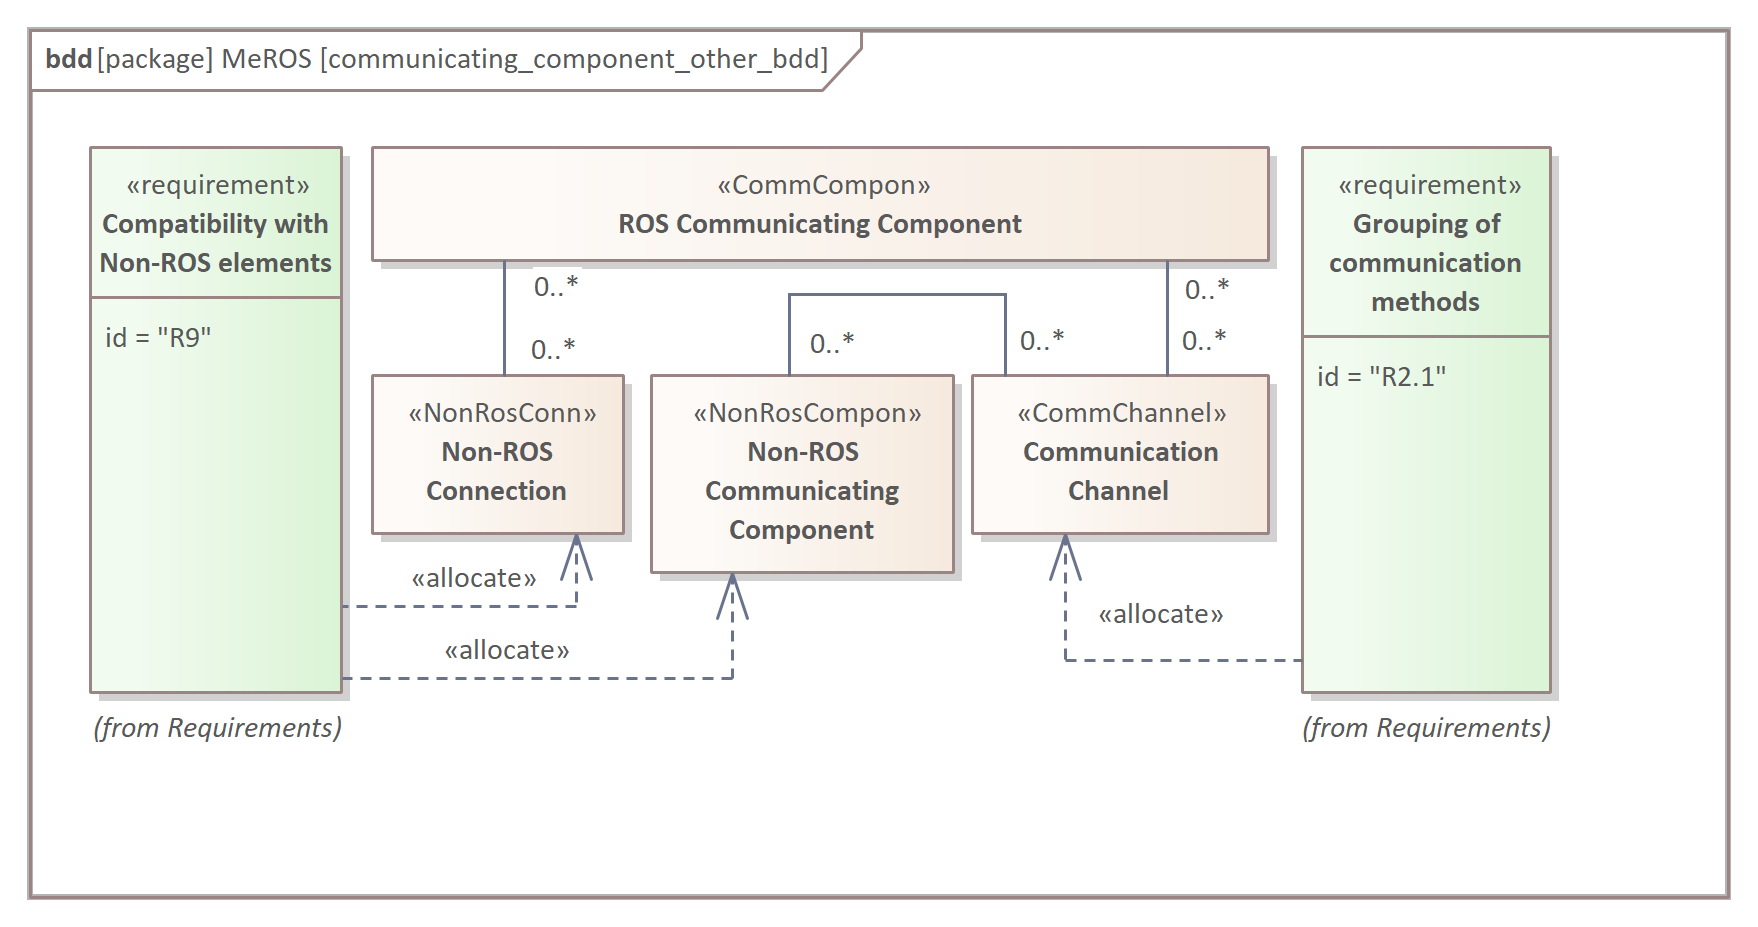
\includegraphics[scale=0.95]{../imgs/meros_pkg/communicating_component_other_bdd.png}}
    \end{center}
    \caption{Communicating Component relations -- aggregates, Non-ROS elements -- bdd.}
    \label{fig:communicating_component_other_bdd}
\end{figure}

Besides standard ROS communication methods, the Non-ROS are also included (e.g., http request) to achieve interfaces with Non-ROS parts of the general system. An Action Data Structure comprises data used by three of five Topics composed in Action, i.e., goal, feedback and result. Two remaining Topics, i.e., cancel and status are standardised.

The Communication Channel \cite{palka2022communication} concept depicted in Fig.~\ref{fig:communication_channel_bdd} is introduced to aggregate specializations of ROS connection (Topic connections, Service connections, and Action connections) as well as Non-ROS Connections. The Communication Channel can also aggregate different Communication Channels.


\begin{figure}[H]
    \centering
    \begin{center}
    {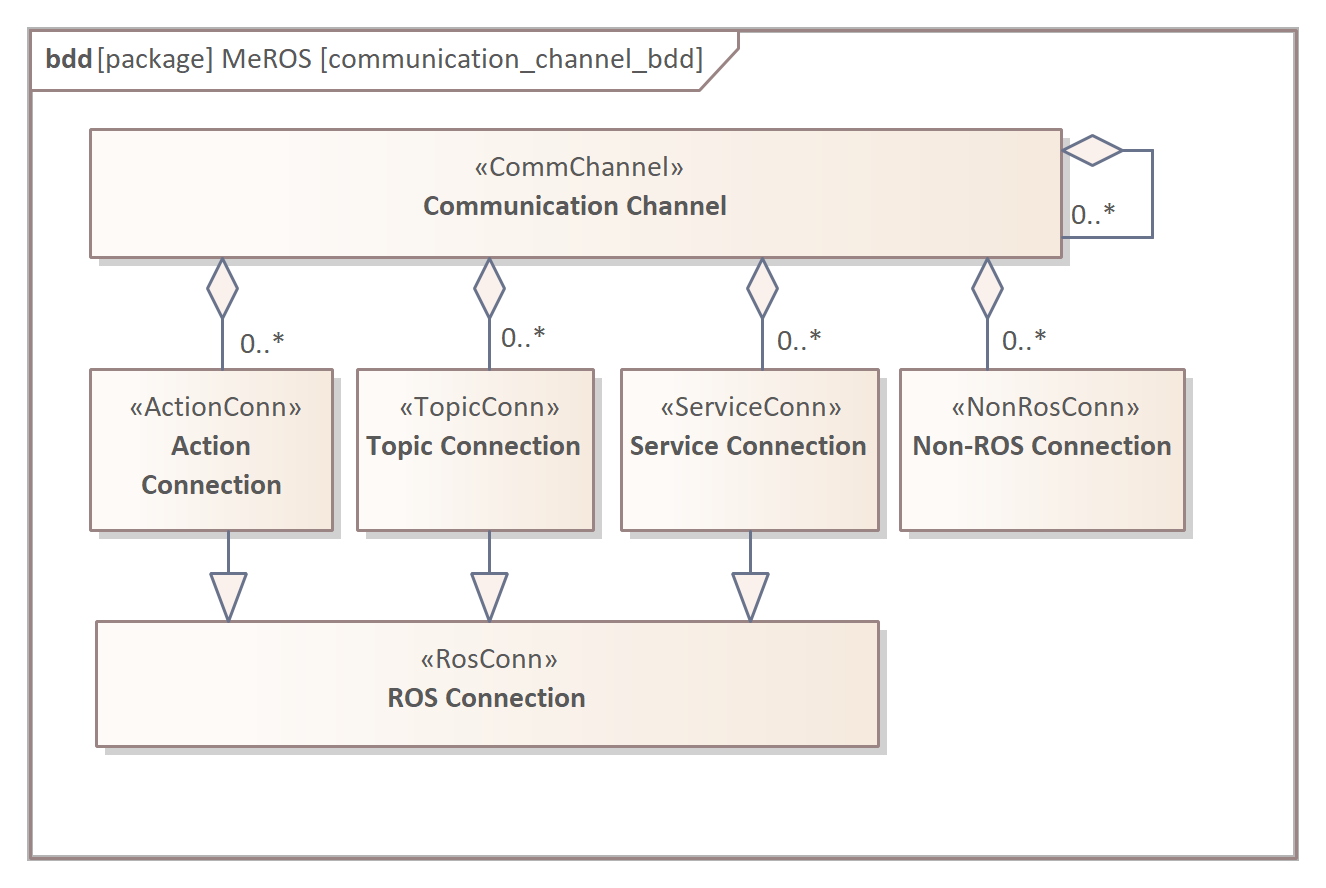
\includegraphics[scale=0.95]{../imgs/meros_pkg/communication_channel_bdd.png}}
    \end{center}
    \caption{Communication Channel -- bdd.}
    \label{fig:communication_channel_bdd}
\end{figure}

The Node (Fig.~\ref{fig:node_bdd}) composes Parameters and Nodelets (the latter in ROS~1). Two specific Nodes are considered in the metamodel: ROS Master and rosout. In ROS~2, Component Container aggregates Nodes executed in a single process.


\begin{figure}[H]
    \centering
    \begin{center}
    {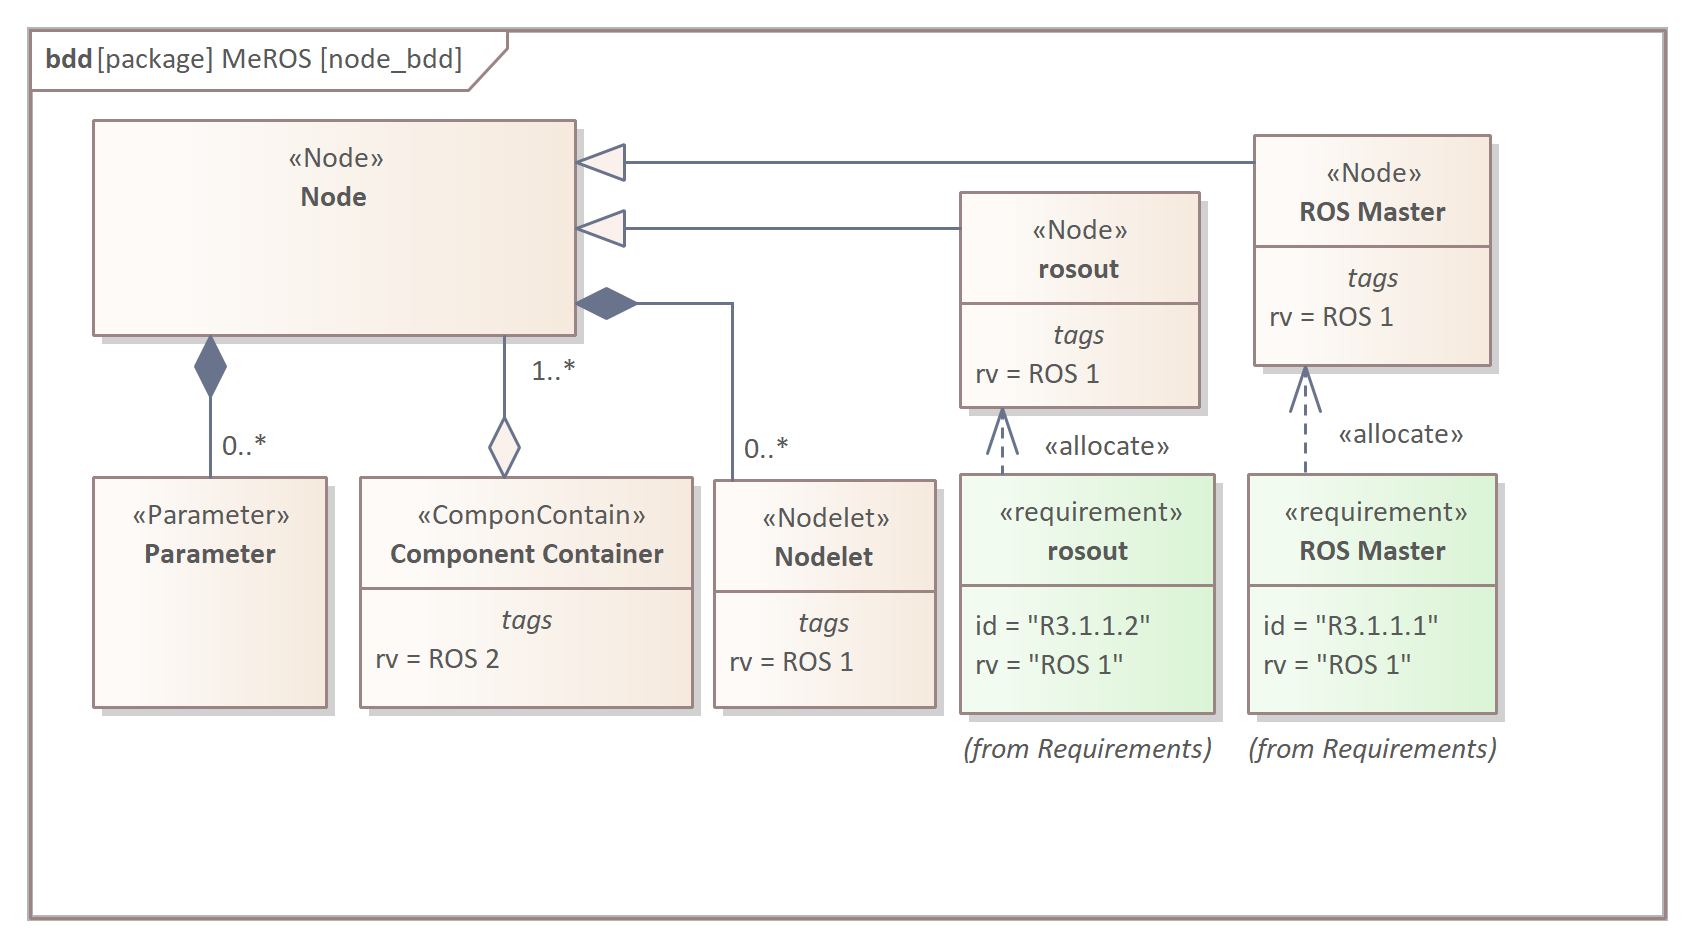
\includegraphics[scale=1.0]{../imgs/meros_pkg/node_bdd.png}}
    \end{center}
    \caption{Node -- bdd.}
    \label{fig:node_bdd}
\end{figure}

The Intrasystem (Fig.~\ref{fig:intrasystem_bdd}) composes ROS and Non-ROS Communicating Component specializations as well as Connections between them. A Parameter block is introduced also for ROS~1. In ROS~2, due to safety reasons, Parameter is composed only into Nodes. Optionally Intrasystem composes the other Intrasystems.


\begin{figure}[H]
    \centering
    \begin{center}
    {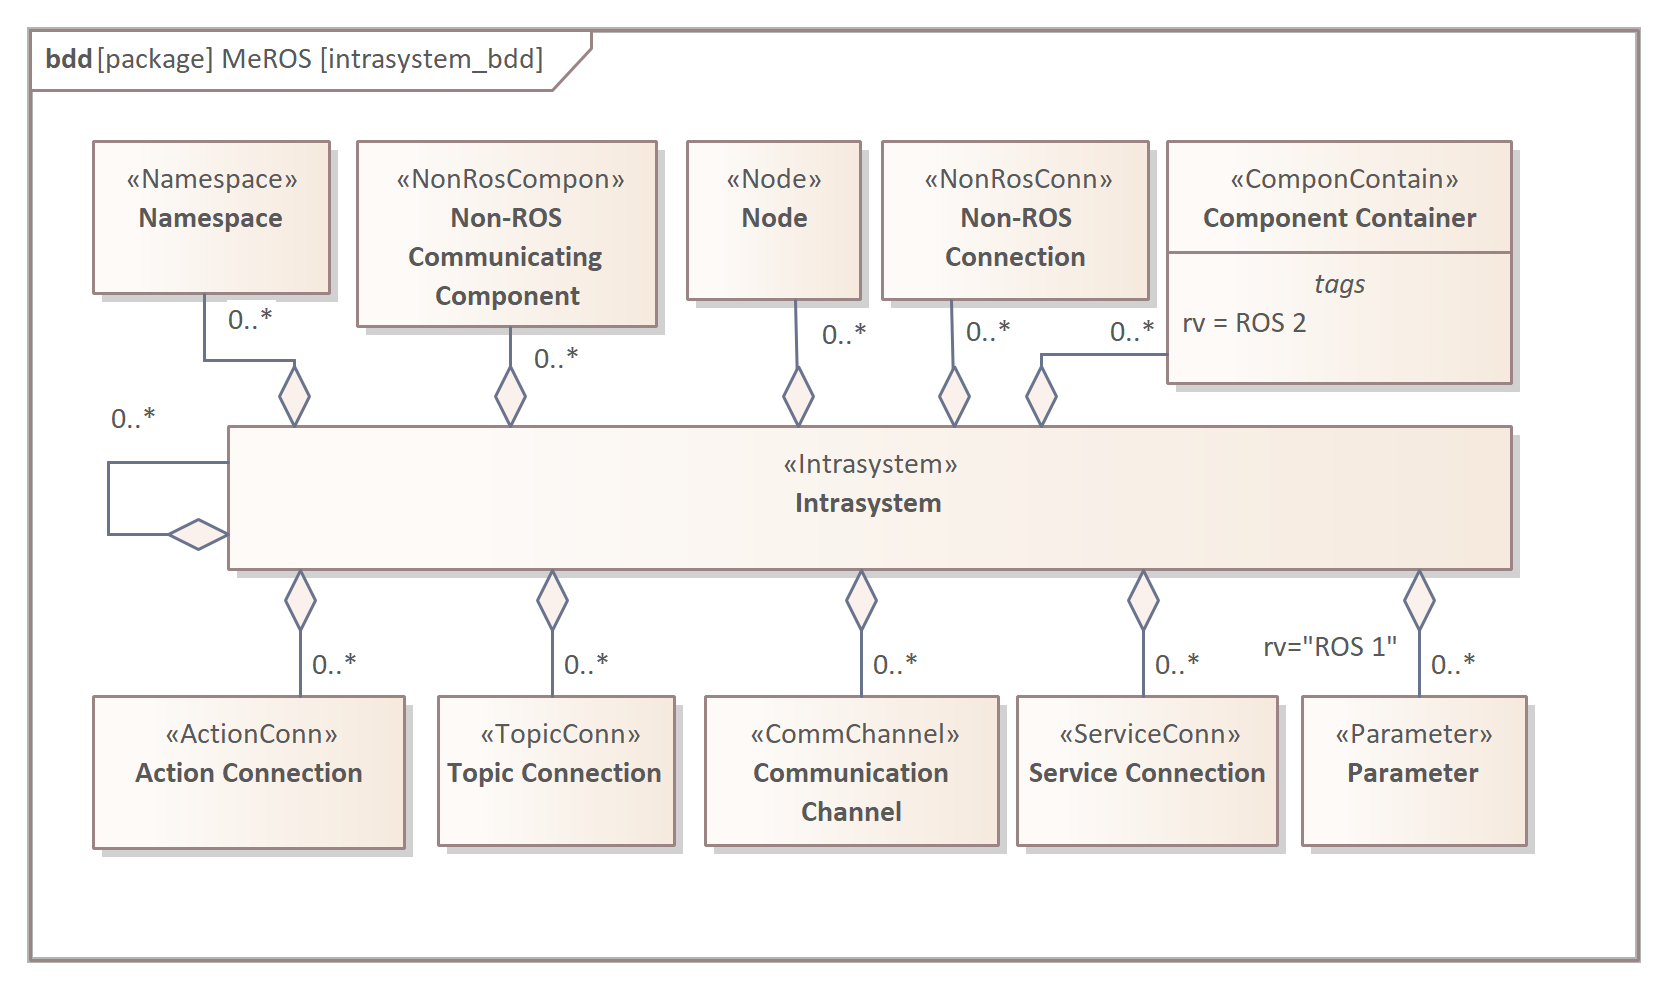
\includegraphics[scale=1.0]{../imgs/meros_pkg/intrasystem_bdd.png}}
    \end{center}
    \caption{Intrasystem compositions -- bdd.}
    \label{fig:intrasystem_bdd}
\end{figure}

The Running System (Fig.~\ref{fig:running_system_bdd}) is a specialisation of the Intrasystem that can be executed. Hence, two Nodes are needed for ROS~1: rosout and ROS master.
It should be noted that although MeROS could be classified as PSM, the initial, general system description with Communications Channels and Intrasystems corresponds to PIM specification. Then, the detailing of these aggregates corresponds to the transition from PIM to PSM.


\begin{figure}[H]
    \centering
    \begin{center}
    {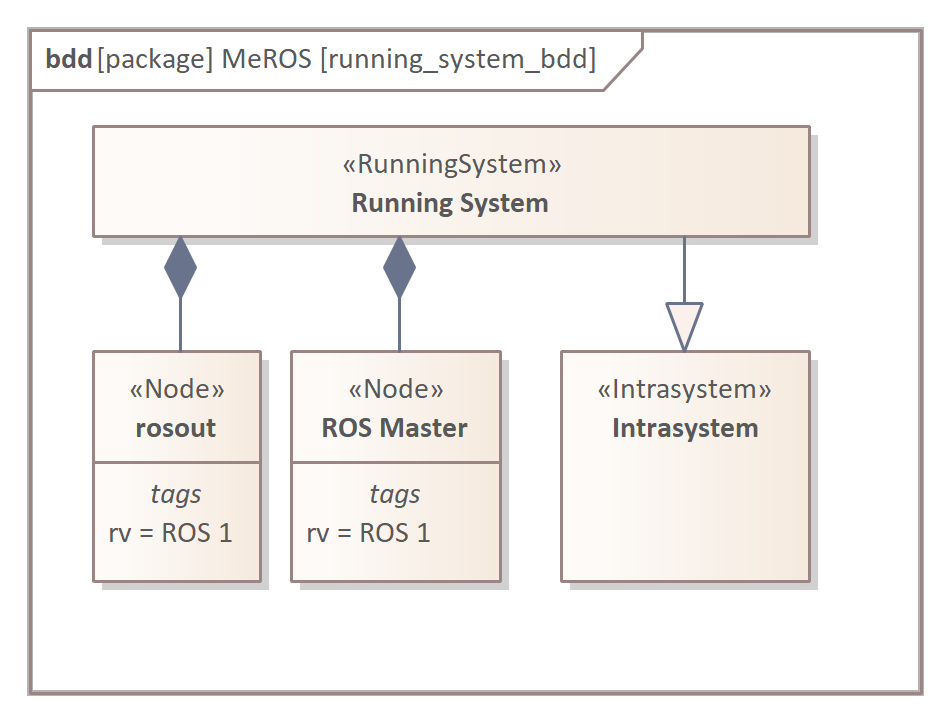
\includegraphics[scale=1.1]{../imgs/meros_pkg/running_system_bdd.png}}
    \end{center}
    \caption{Running System compositions -- bdd.}
    \label{fig:running_system_bdd}
\end{figure}

The way Communicating Components use various types of connections is presented in Fig.~\ref{fig:running_system_communication_bdd}. Both ROS and Non-ROS Communicating Components can communicate via Non-ROS Connections, but only ROS Communicating Components use ROS Connections.


\begin{figure}[H]
    \centering
    \begin{center}
    {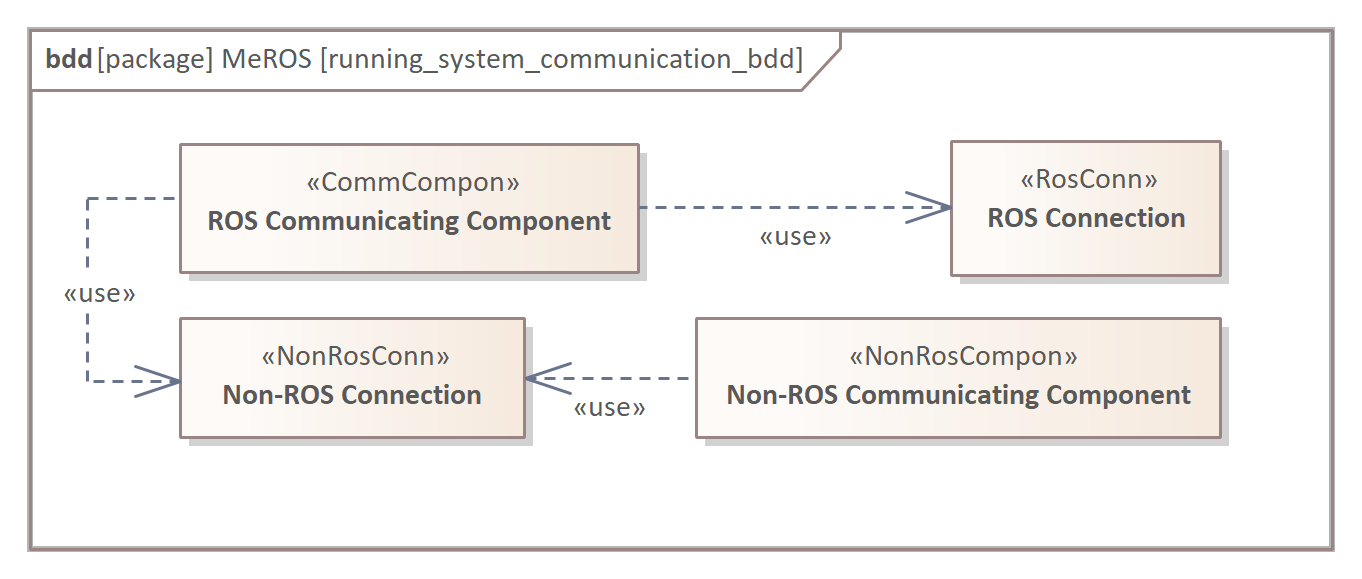
\includegraphics[scale=1.1]{../imgs/meros_pkg/running_system_communication_bdd.png}}
    \end{center}
    \caption{Running System communication -- bdd.}
    \label{fig:running_system_communication_bdd}
\end{figure}

\pagebreak

The Namespace (Fig.~\ref{fig:namespace_bdd}) aggregates elements of the Intrasystem, but only ROS related. In opposition to the Intrasystem, the Namespace does not specialise Communicating Component. Hence, it can not act as Communicating Component.


\begin{figure}[H]
    \centering
    \begin{center}
    {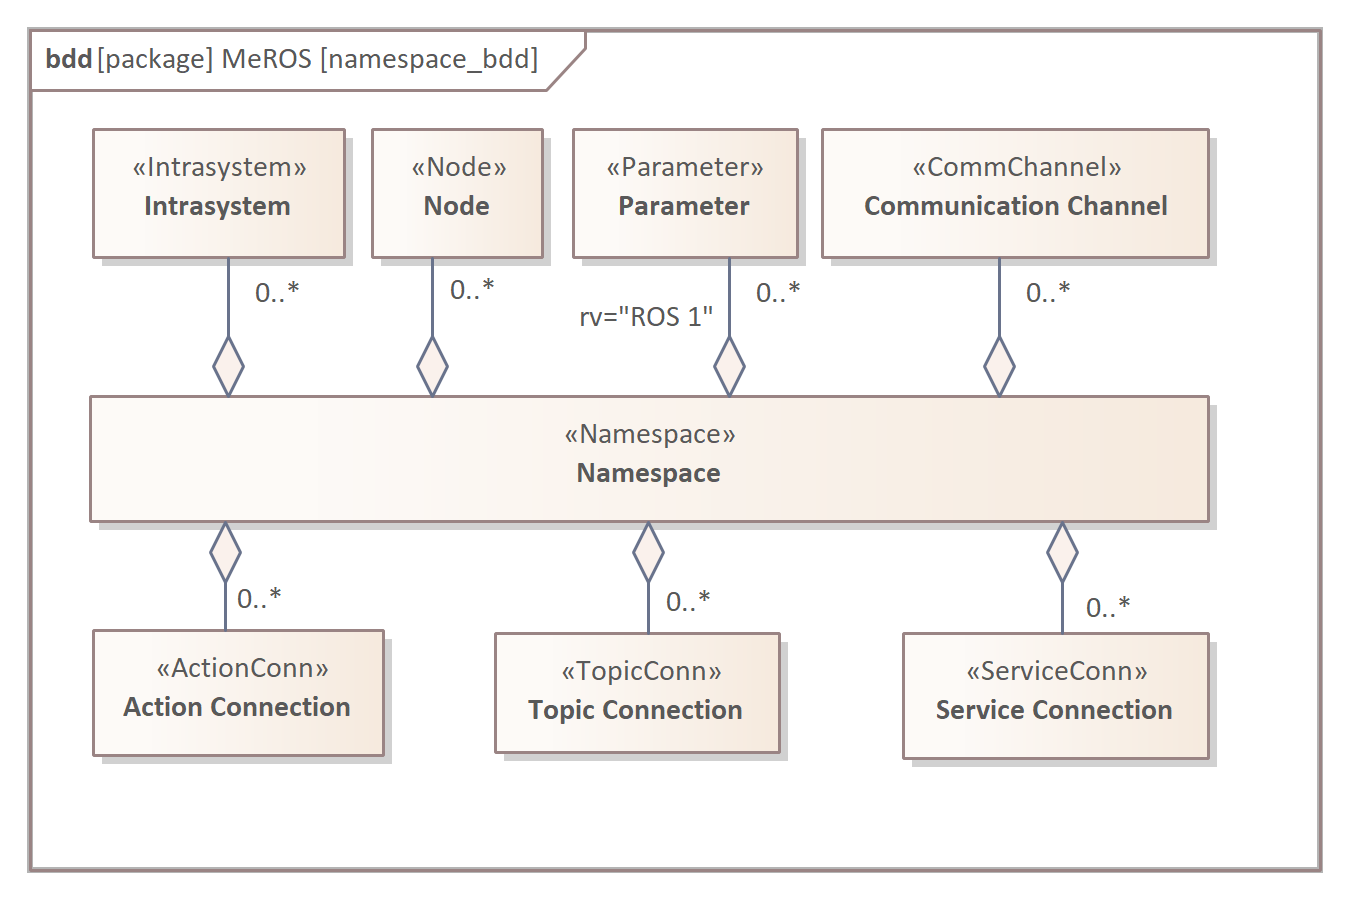
\includegraphics[scale=1.0]{../imgs/meros_pkg/namespace_bdd.png}}
    \end{center}
    \caption{Namespace composition -- bdd.}
    \label{fig:namespace_bdd}
\end{figure}


The Package (Fig.~\ref{fig:ros_package_bdd}) composes the files related to general ROS concepts such as Node source codes, communication structures definitions, etc. It should be noted that in case of Actions, specific communication structures definitions are stored in Action Data Structures. The Misc <<block>> relates to other ROS and Non-ROS files, e.g., roslaunch configuration, obligatory package.xml, CMakeLists.txt. The Metapackage is introduced for conformity with the latest ROS~1 releases [R7] as well as ROS~2.


\begin{figure}[H]
    \centering
    \begin{center}
    {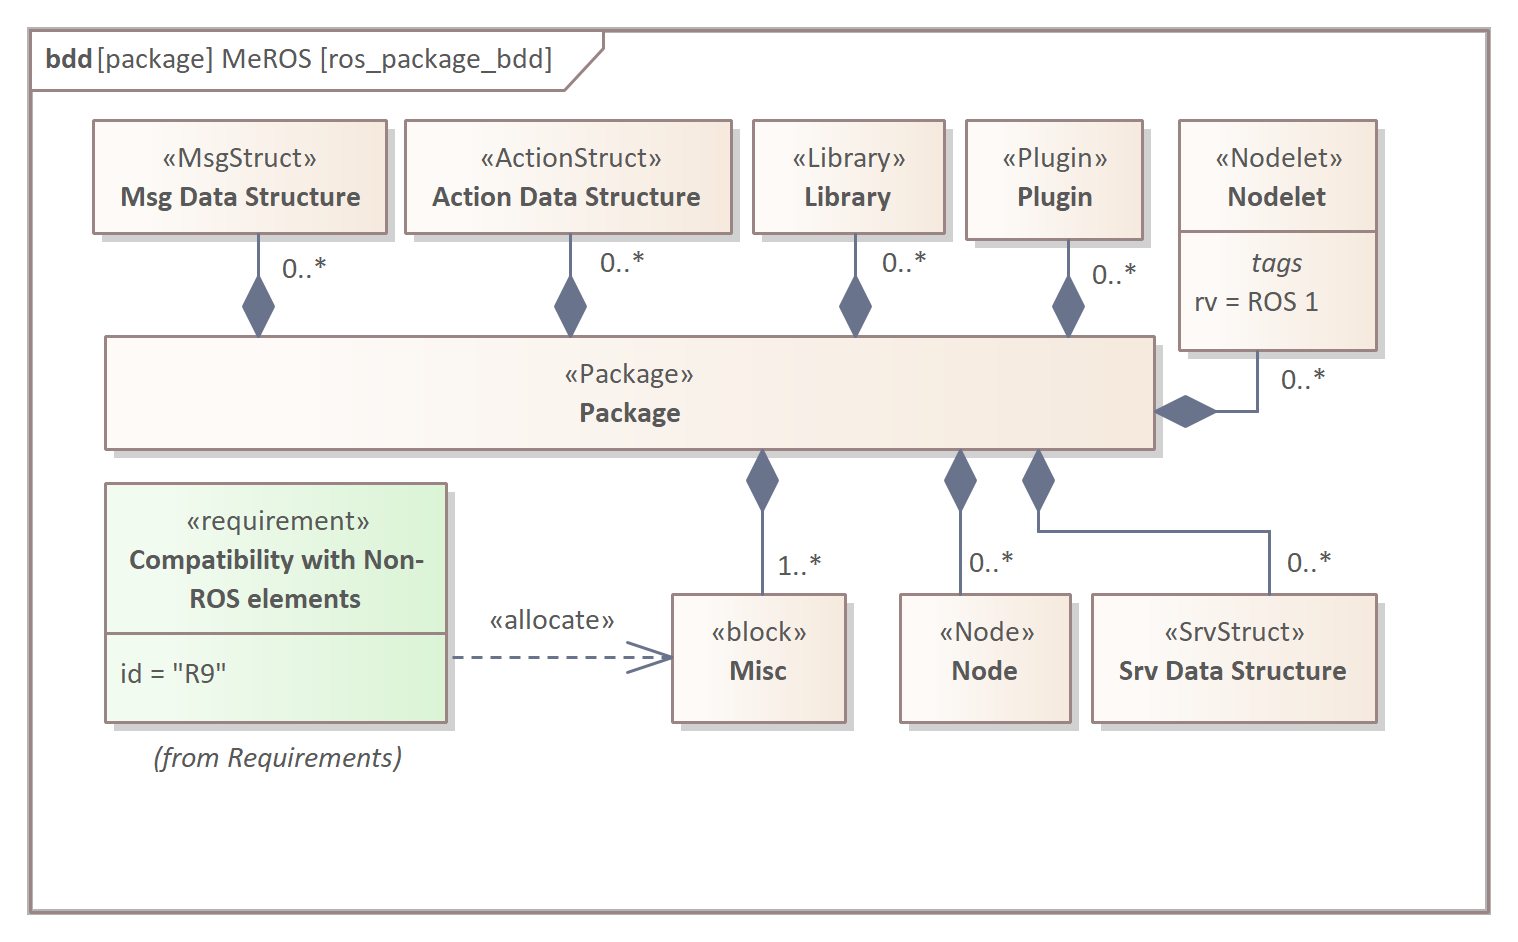
\includegraphics[scale=1.0]{../imgs/meros_pkg/ros_package_bdd.png}}
    \end{center}
    \caption{ROS Package composition -- bdd.}
    \label{fig:ros_package_bdd}
\end{figure}

The Workspace (Fig.~\ref{fig:ros_workspace_bdd}) contains of Packages that compose the files related to general ROS concepts such as Node source codes, communication structures definitions, etc. As Workspace has a specific file-system nature, Group of Packages were introduced as a more general component. The Repository plays a similar role to the Workspace, but reflects the place where sources are stored.


\begin{figure}[H]
    \centering
    \begin{center}
    {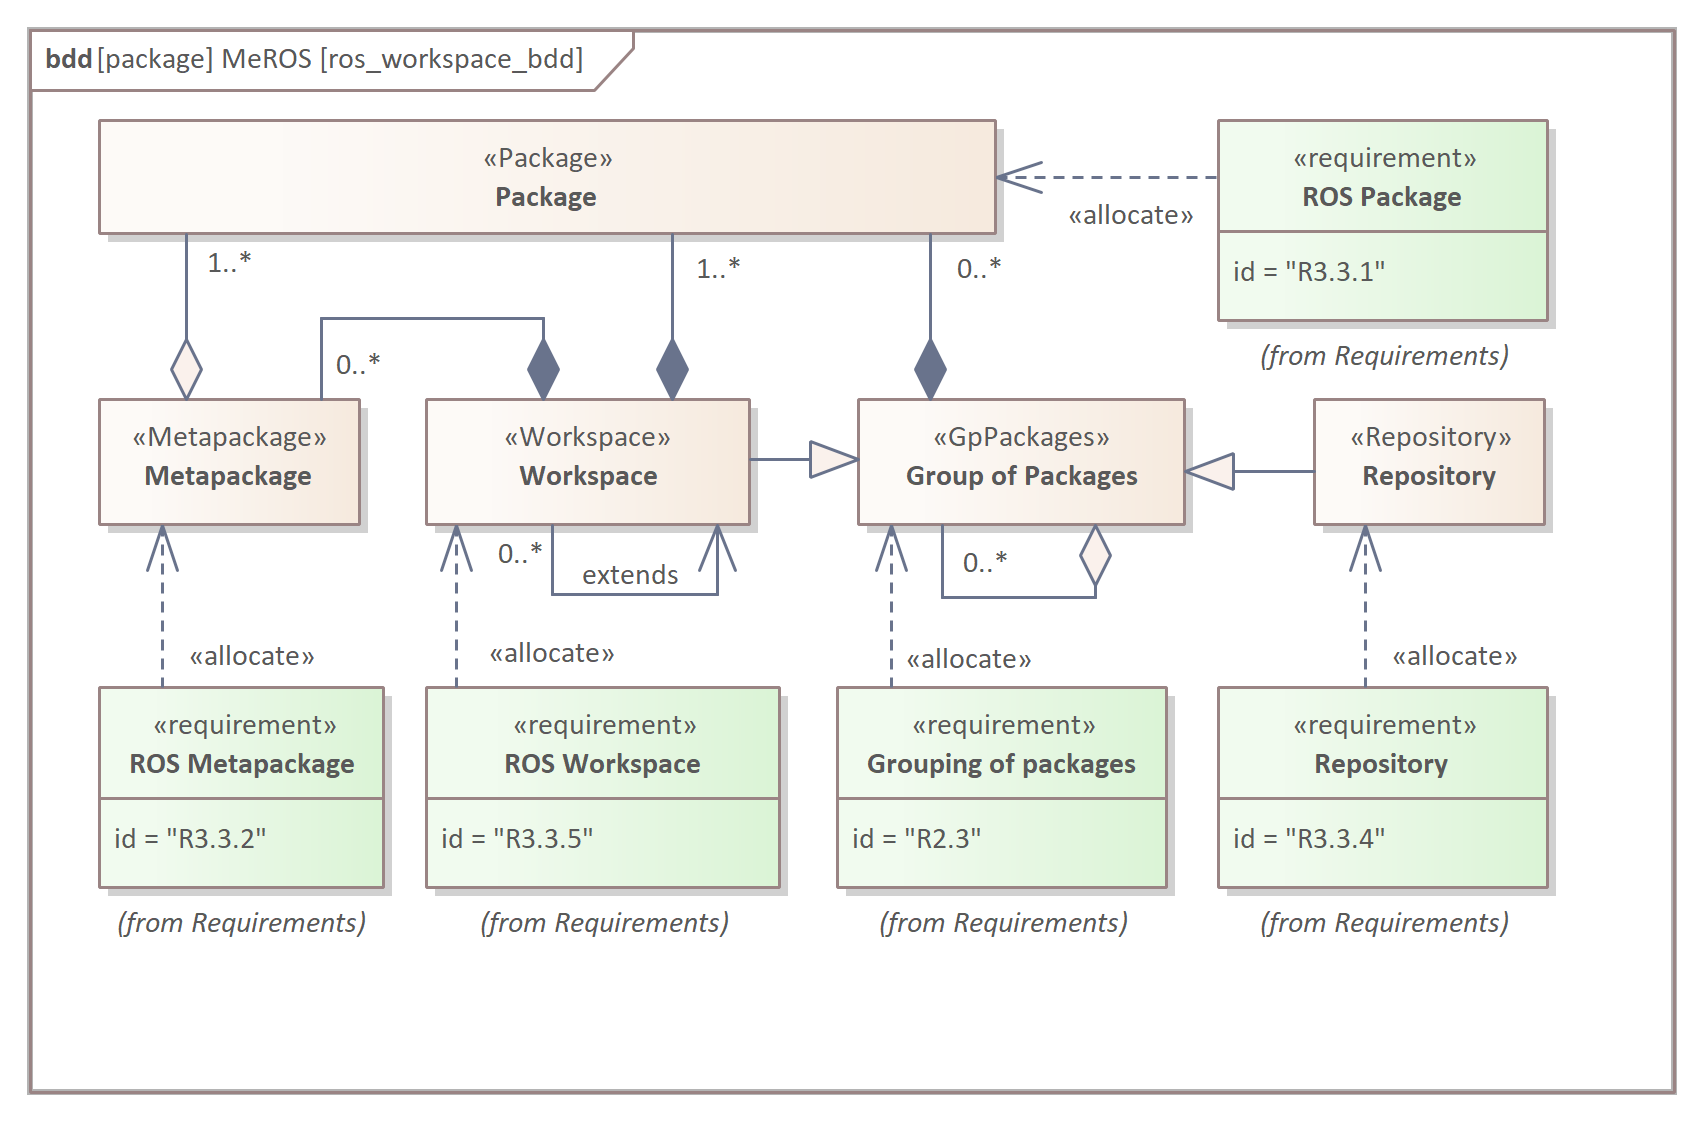
\includegraphics[scale=1]{../imgs/meros_pkg/ros_workspace_bdd.png}}
    \end{center}
    \caption{ROS Workspace composition -- bdd.}
    \label{fig:ros_workspace_bdd}
\end{figure}







\subsection{Communication}
\label{sec:metamodel-communication}

This section depicts the behavioural and structural aspects of communication in the system. The previous section considers block definition diagrams (bdd). In the following part, the internal block diagrams (ibd) and behavioural diagrams are discussed. The goal is to present three modes of communication: Topic [R4.1] (sec.~\ref{sec:metamodel-topic}), Service [R4.2] (sec.~\ref{sec:metamodel-service}) and Action [R4.3] (sec.~\ref{sec:metamodel-action}). It should be noted that the concept of presentation of communication with and without a dedicated communication component is illustrated on communication with Topics but can also be applied to Services, Actions and Communication Channels.

\pagebreak
\subsubsection{Topic}
\label{sec:metamodel-topic}

Fig.~\ref{fig:topic_communication_with_dedicated_component_ibd} presents the ibd diagram of publishers' and subscribers' communication via topics. This diagram uses a dedicated communication component for each Topic [R4.1.1]. There are no general limits to the number of publishers, subscribers and Topics they communicate with.


\begin{figure}[H]
    \centering
    \begin{center}
    {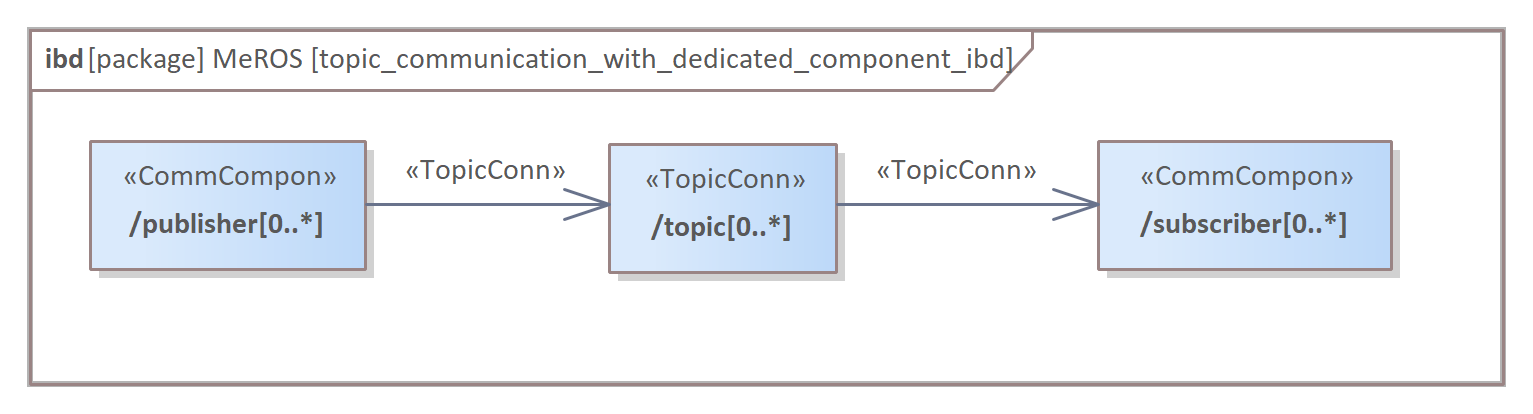
\includegraphics[scale=1.0]{../imgs/meros_pkg/topic_communication_with_dedicated_component_ibd.png}}
    \end{center}
    \caption{Topics with dedicated communication components -- all components -- ibd.}
    \label{fig:topic_communication_with_dedicated_component_ibd}
\end{figure}

Thanks to a dedicated component to represent communication, the diagram in Fig.~\ref{fig:topic_communication_with_dedicated_component_ibd} can be split into two considering publisher (Fig.~\ref{fig:topic_split_publisher_ibd}) and subscriber (Fig.~\ref{fig:topic_split_subscriber_ibd}) separately, without losing information. It is especially useful when system fragments are presented after its decomposition that subdivides communication channels.


\begin{figure}[H]
    \centering
    \begin{center}
    {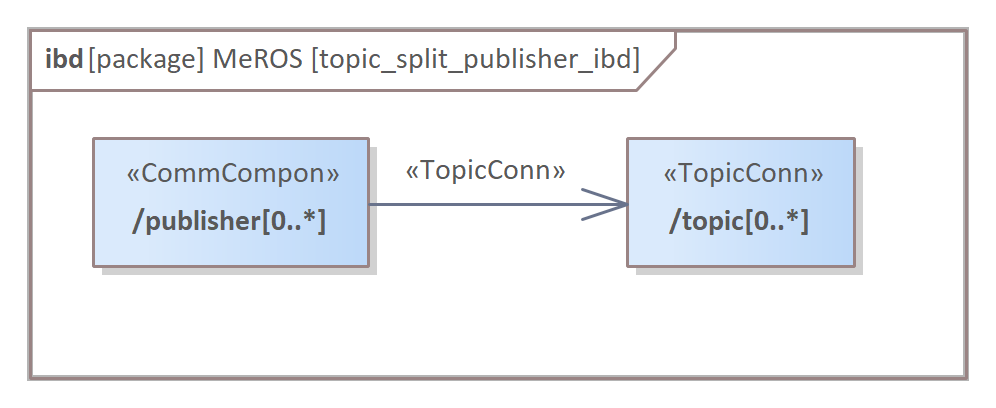
\includegraphics[scale=1.0]{../imgs/meros_pkg/topic_split_publisher_ibd.png}}
    \end{center}
    \caption{Topics with dedicated communication components -- publisher -- ibd.}
    \label{fig:topic_split_publisher_ibd}
\end{figure}


\begin{figure}[H]
    \centering
    \begin{center}
    {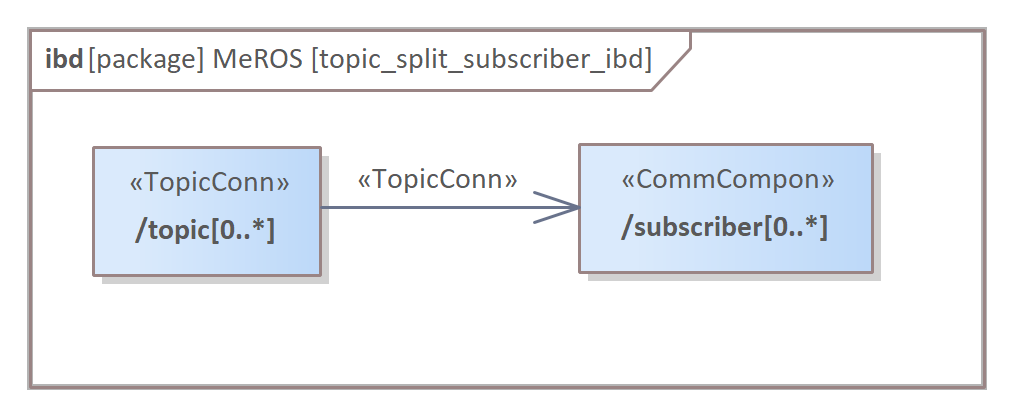
\includegraphics[scale=1.0]{../imgs/meros_pkg/topic_split_subscriber_ibd.png}}
    \end{center}
    \caption{Topics with dedicated communication components -- subscriber -- ibd.}
    \label{fig:topic_split_subscriber_ibd}
\end{figure}


\pagebreak

Fig. \ref{fig:topic_communication_with_dedicated_component_sd} depicts the corresponding sequence diagram. Publishers send a message through Topics to the subscribers. The incoming message cause the subscriber to execute the callback function. 	Fig.~\ref{fig:topic_communication_without_dedicated_component_ibd} and Fig.~\ref{fig:topic_communication_without_dedicated_component_sd} present an alternative approach to depict the system communicating via topics. In this case, no dedicated communication components are used [R4.1.2].

\begin{figure}[H]
    \centering
    \begin{center}
    {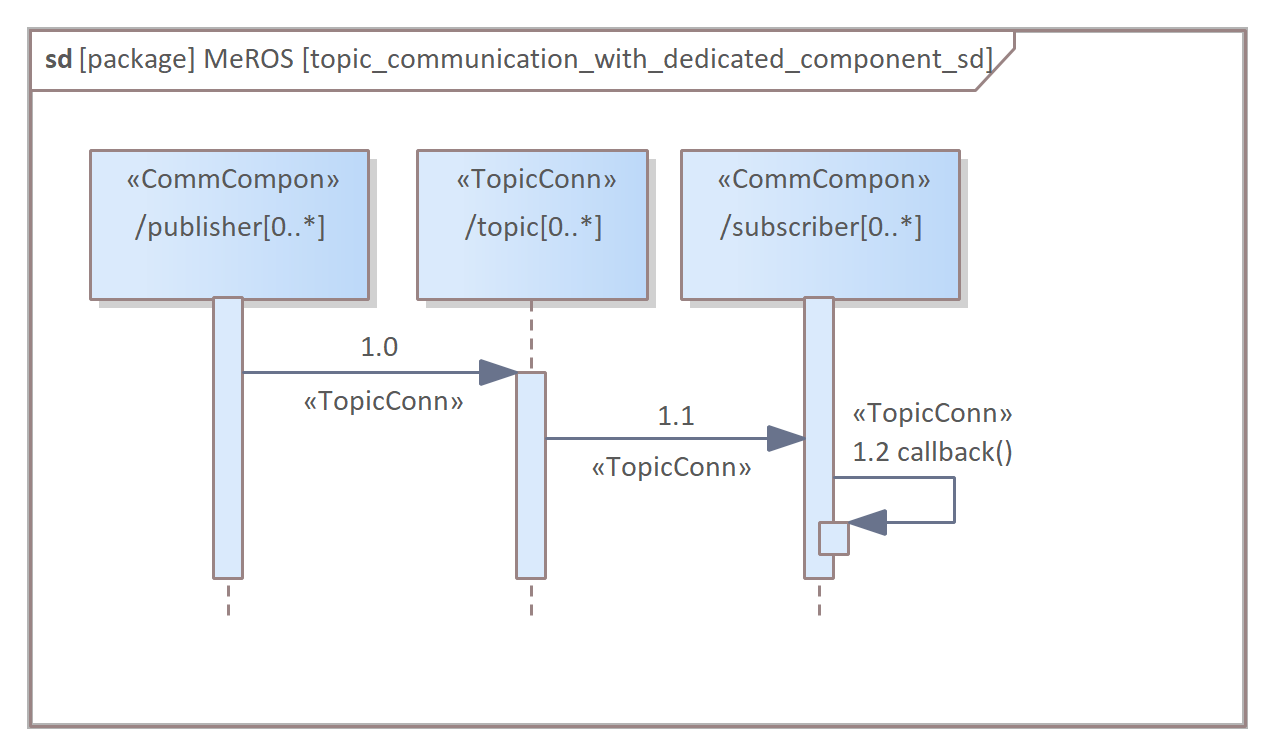
\includegraphics[scale=1.0]{../imgs/meros_pkg/topic_communication_with_dedicated_component_sd.png}}
    \end{center}
    \caption{Topics with dedicated communication components -- sd.}
    \label{fig:topic_communication_with_dedicated_component_sd}
\end{figure}


\begin{figure}[H]
    \centering
    \begin{center}
    {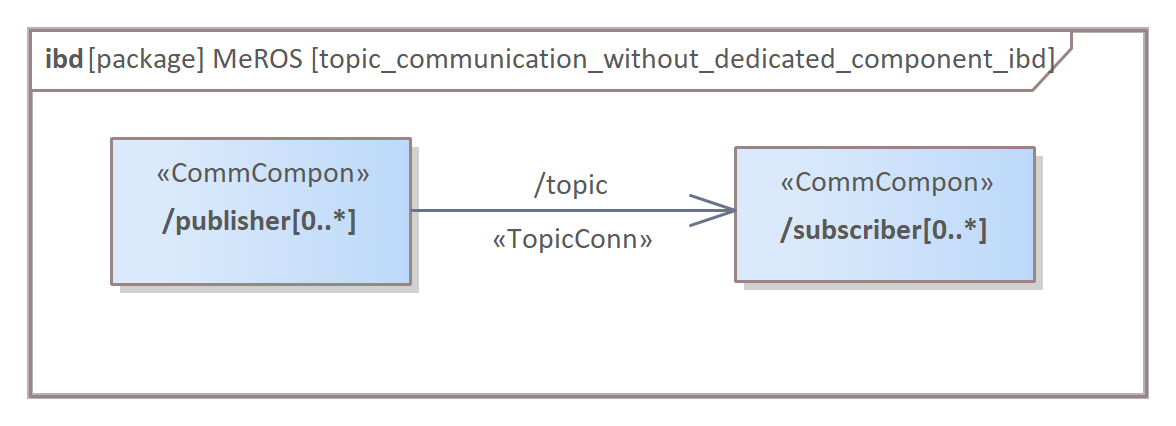
\includegraphics[scale=1.0]{../imgs/meros_pkg/topic_communication_without_dedicated_component_ibd.png}}
    \end{center}
    \caption{Topics without dedicated communication components -- ibd.}
    \label{fig:topic_communication_without_dedicated_component_ibd}
\end{figure}

\begin{figure}[H]
    \centering
    \begin{center}
    {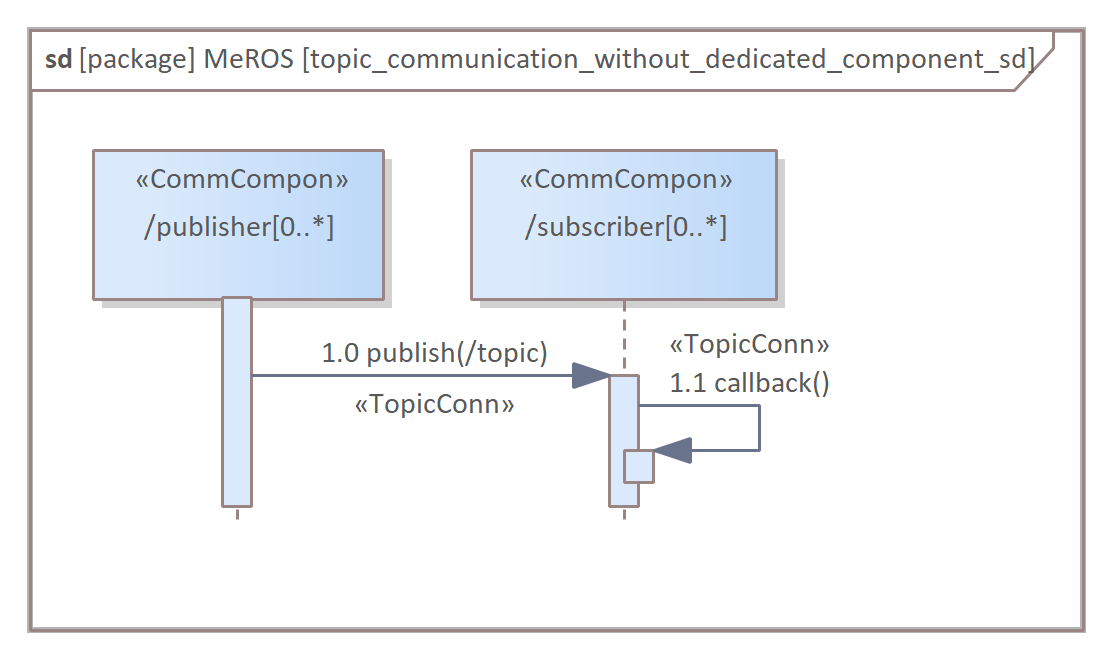
\includegraphics[scale=1.0]{../imgs/meros_pkg/topic_communication_without_dedicated_component_sd.png}}
    \end{center}
    \caption{Topics without dedicated communication components -- sd.}
    \label{fig:topic_communication_without_dedicated_component_sd}
\end{figure}

\subsubsection{Service}
\label{sec:metamodel-service}

For each ROS Service, there is at most one server and a~number of clients (Fig.~\ref{fig:service_communication_ibd} and Fig.~\ref{fig:service_communication_sd}). Service-type communication is bidirectional and realises RPC (remote procedure call).


\begin{figure}[H]
    \centering
    \begin{center}
    {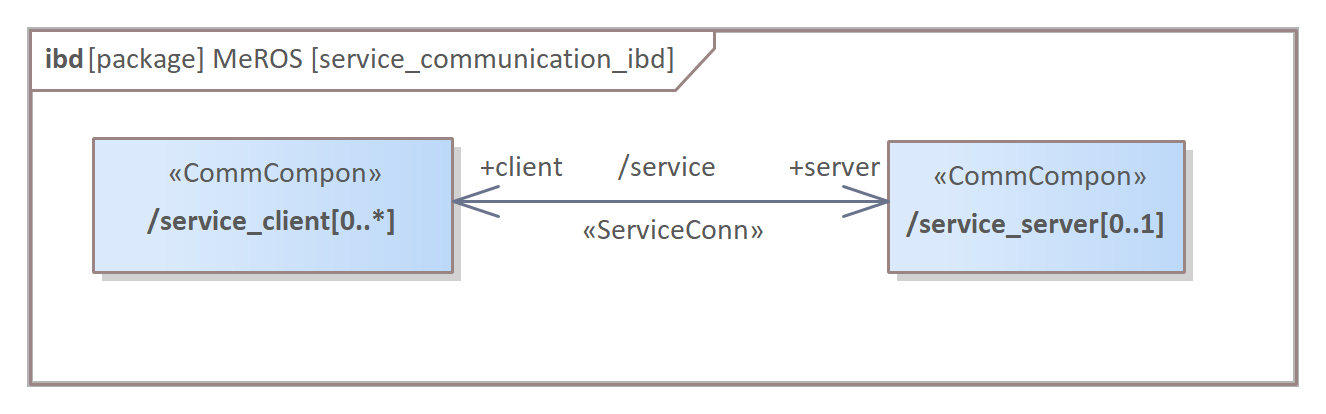
\includegraphics[scale=1.0]{../imgs/meros_pkg/service_communication_ibd.png}}
    \end{center}
    \caption{Service-based communication -- ibd.}
    \label{fig:service_communication_ibd}
\end{figure}


\begin{figure}[H]
    \centering
    \begin{center}
    {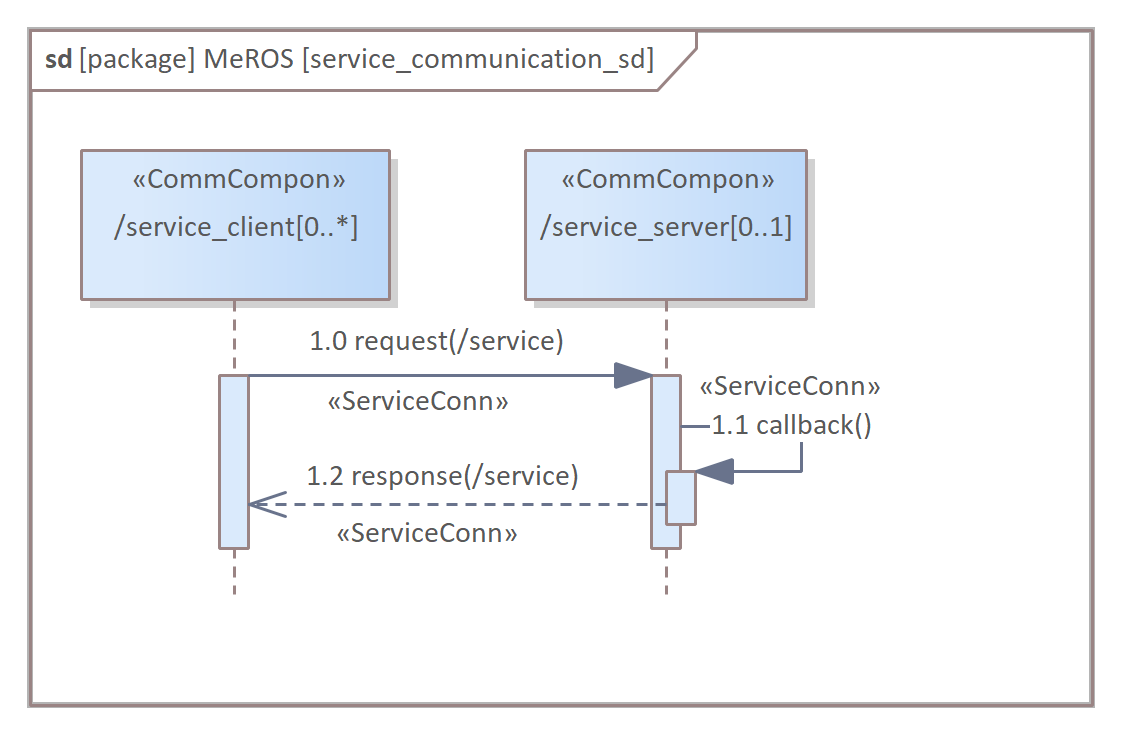
\includegraphics[scale=1.0]{../imgs/meros_pkg/service_communication_sd.png}}
    \end{center}
    \caption{Service-based communication -- sd.}
    \label{fig:service_communication_sd}
\end{figure}


\subsubsection{Action}
\label{sec:metamodel-action}

ROS Action communication's general, simplified structure (Fig.~\ref{fig:action_communication_compact_ibd}) is analogous to ROS Service. These type of presentation is universal for ROS~1 and ROS~2.


\begin{figure}[H]
    \centering
    \begin{center}
    {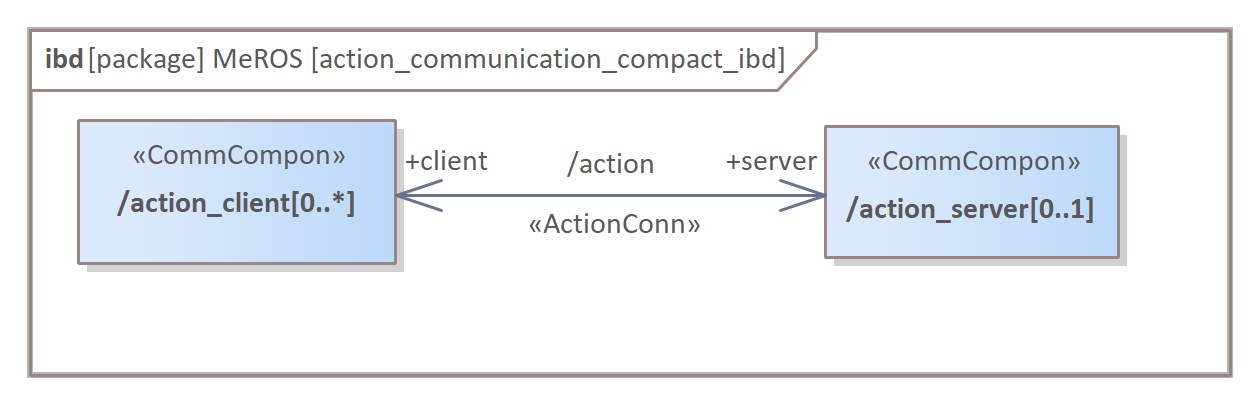
\includegraphics[scale=1.0]{../imgs/meros_pkg/action_communication_compact_ibd.png}}
    \end{center}
    \caption{Action-based communication -- compact representation -- ibd.}
    % https://docs.ros.org/en/foxy/Tutorials/Beginner-CLI-Tools/Understanding-ROS2-Actions/Understanding-ROS2-Actions.html
    \label{fig:action_communication_compact_ibd}
\end{figure}

\pagebreak

An Action (Fig.~\ref{fig:action_communication_detailed_ibd}) is based on several Topics in ROS~1, while on Topics and Services in ROS~2.


\begin{figure}[H]
    \centering
    \begin{center}
    {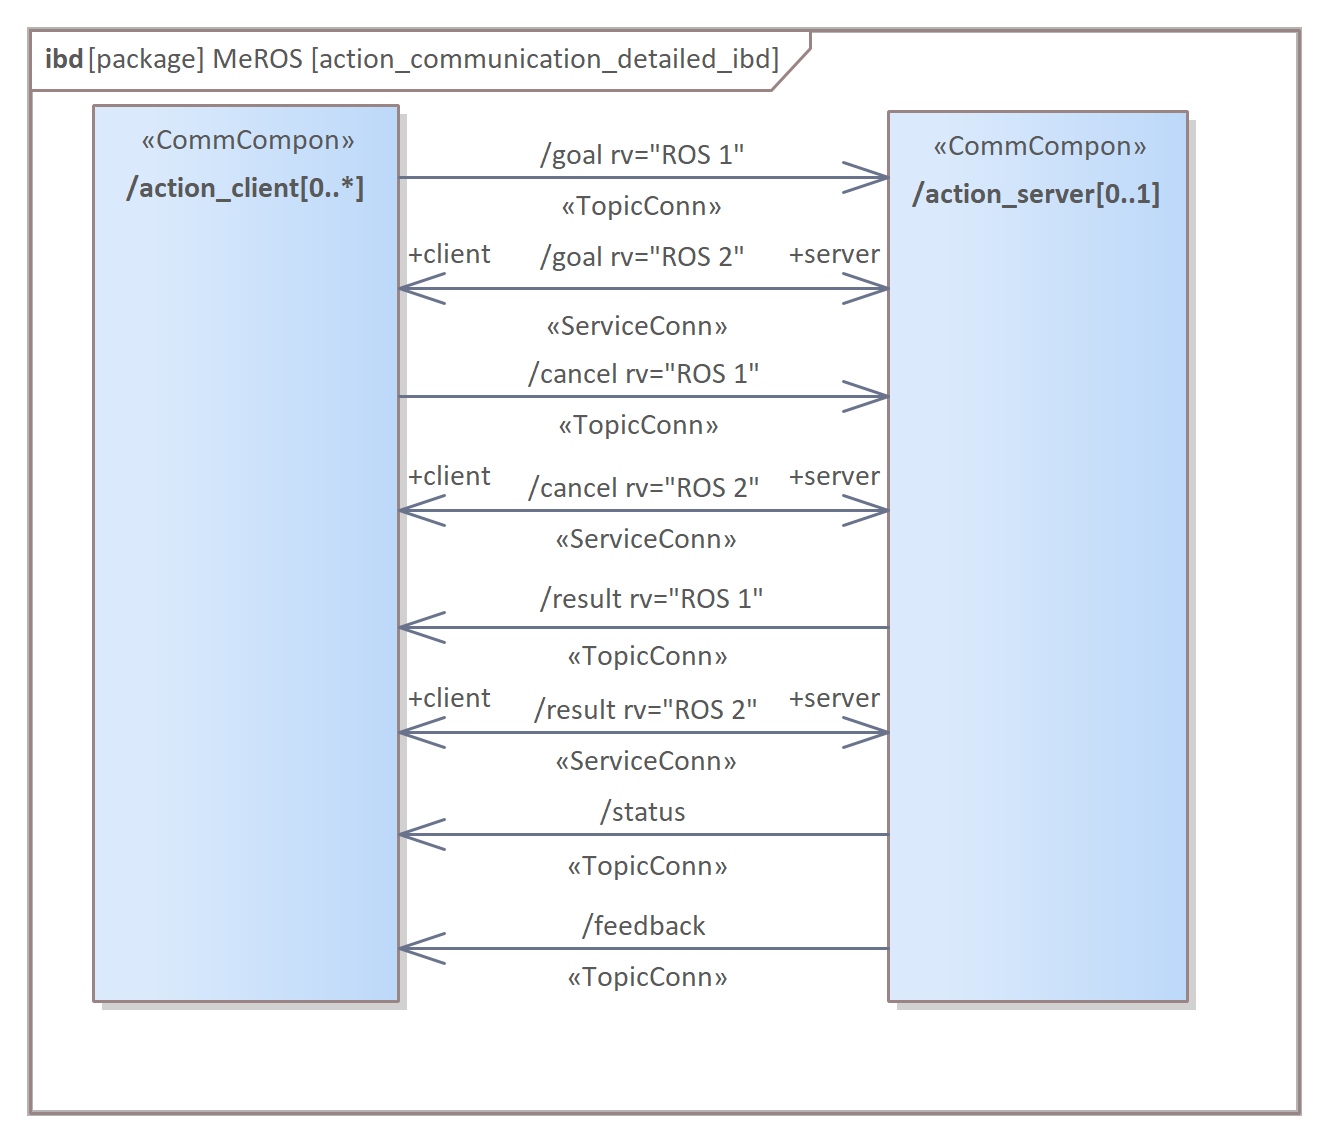
\includegraphics[scale=1.0]{../imgs/meros_pkg/action_communication_detailed_ibd.png}}
    \end{center}
    \caption{Action-based communication -- detailed -- ibd.}
    % https://design.ros2.org/articles/actions.html
    \label{fig:action_communication_detailed_ibd}
\end{figure}

In practice, to present an action-related communication compactly on sd diagram (Fig.~\ref{fig:action_communication_compact_sd}) particular Topics and Services can be generalised as a~request (for /goal and /cancel) and a~response (for /status, /feedback and /result). It should be noted that this diagram presents the Action communication sequence in a simplified way.

\begin{figure}[H]
    \centering
    \begin{center}
    {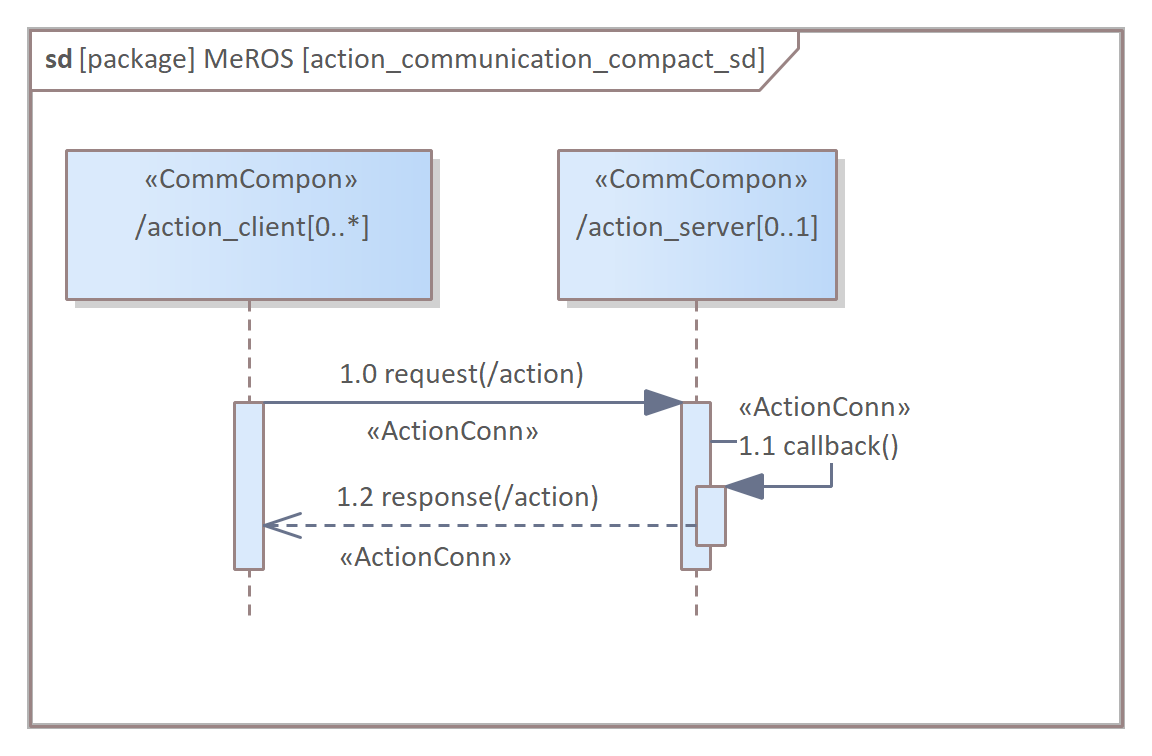
\includegraphics[scale=1.0]{../imgs/meros_pkg/action_communication_compact_sd.png}}
    \end{center}
    \caption{Action-based communication sequence -- compact presentation -- sd.}
    \label{fig:action_communication_compact_sd}
\end{figure}

\pagebreak

The detailed behaviour of the Action server and Action client in ROS~1 is specified by state machines \footnote{\url{http://wiki.ros.org/actionlib/DetailedDescription}}. ROS~2 Action server and Action client behaviour is analogous. Here, these two state machines are depicted in stm diagrams. In the description, in addition to the original ROS wiki presentation, the Topics are directly mentioned both in transitions and states actions.
Fig.~\ref{fig:ros1_action_server_stm} depicts the ROS~1 Action server state machine.
Its transitions depend on the new messages sent by the Action client or internal predicates.

\begin{figure}[H]
    \centering
    \begin{center}
    {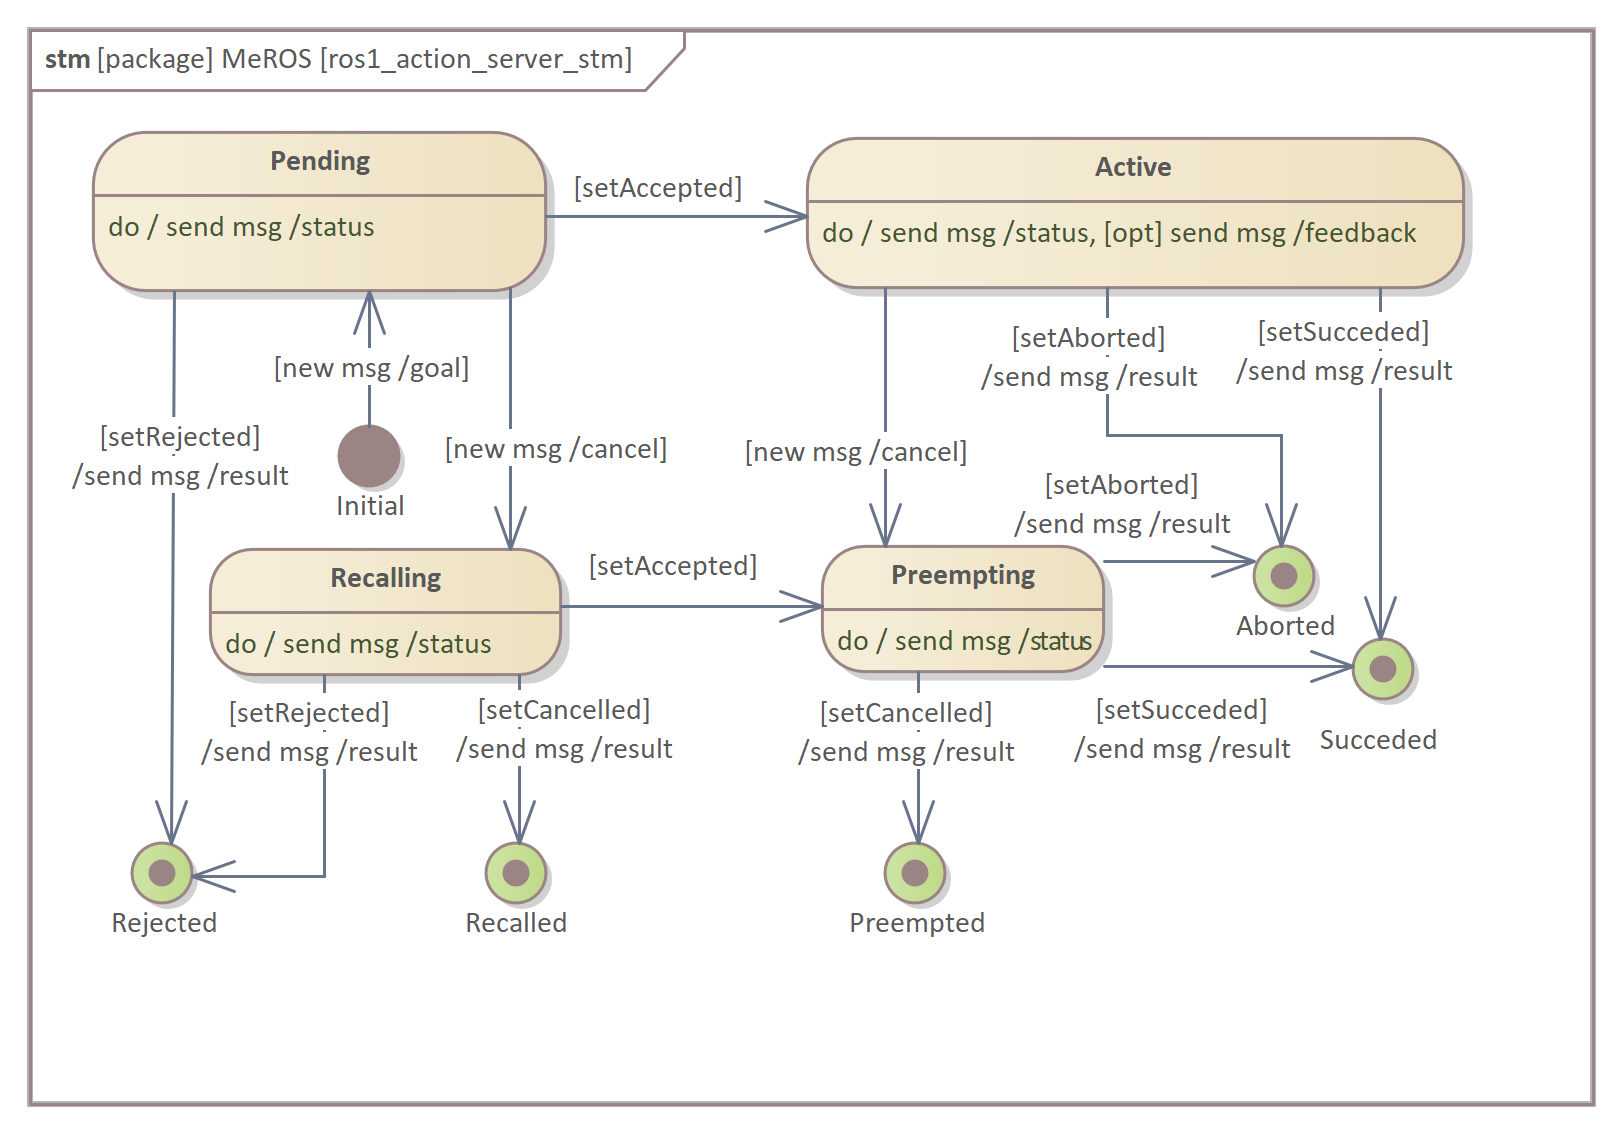
\includegraphics[scale=1.1]{../imgs/meros_pkg/ros1_action_server_stm.png}}
    \end{center}
    \caption{ROS~1 Action server -- stm.}
    \label{fig:ros1_action_server_stm}
\end{figure}

\pagebreak


The ROS~1 Action client state machine (Fig.~\ref{fig:ros1_action_client_stm}) depends on the server state provided by the Action server in /status Topic and internal predicates.

\begin{figure}[H]
    \centering
    \begin{center}
    {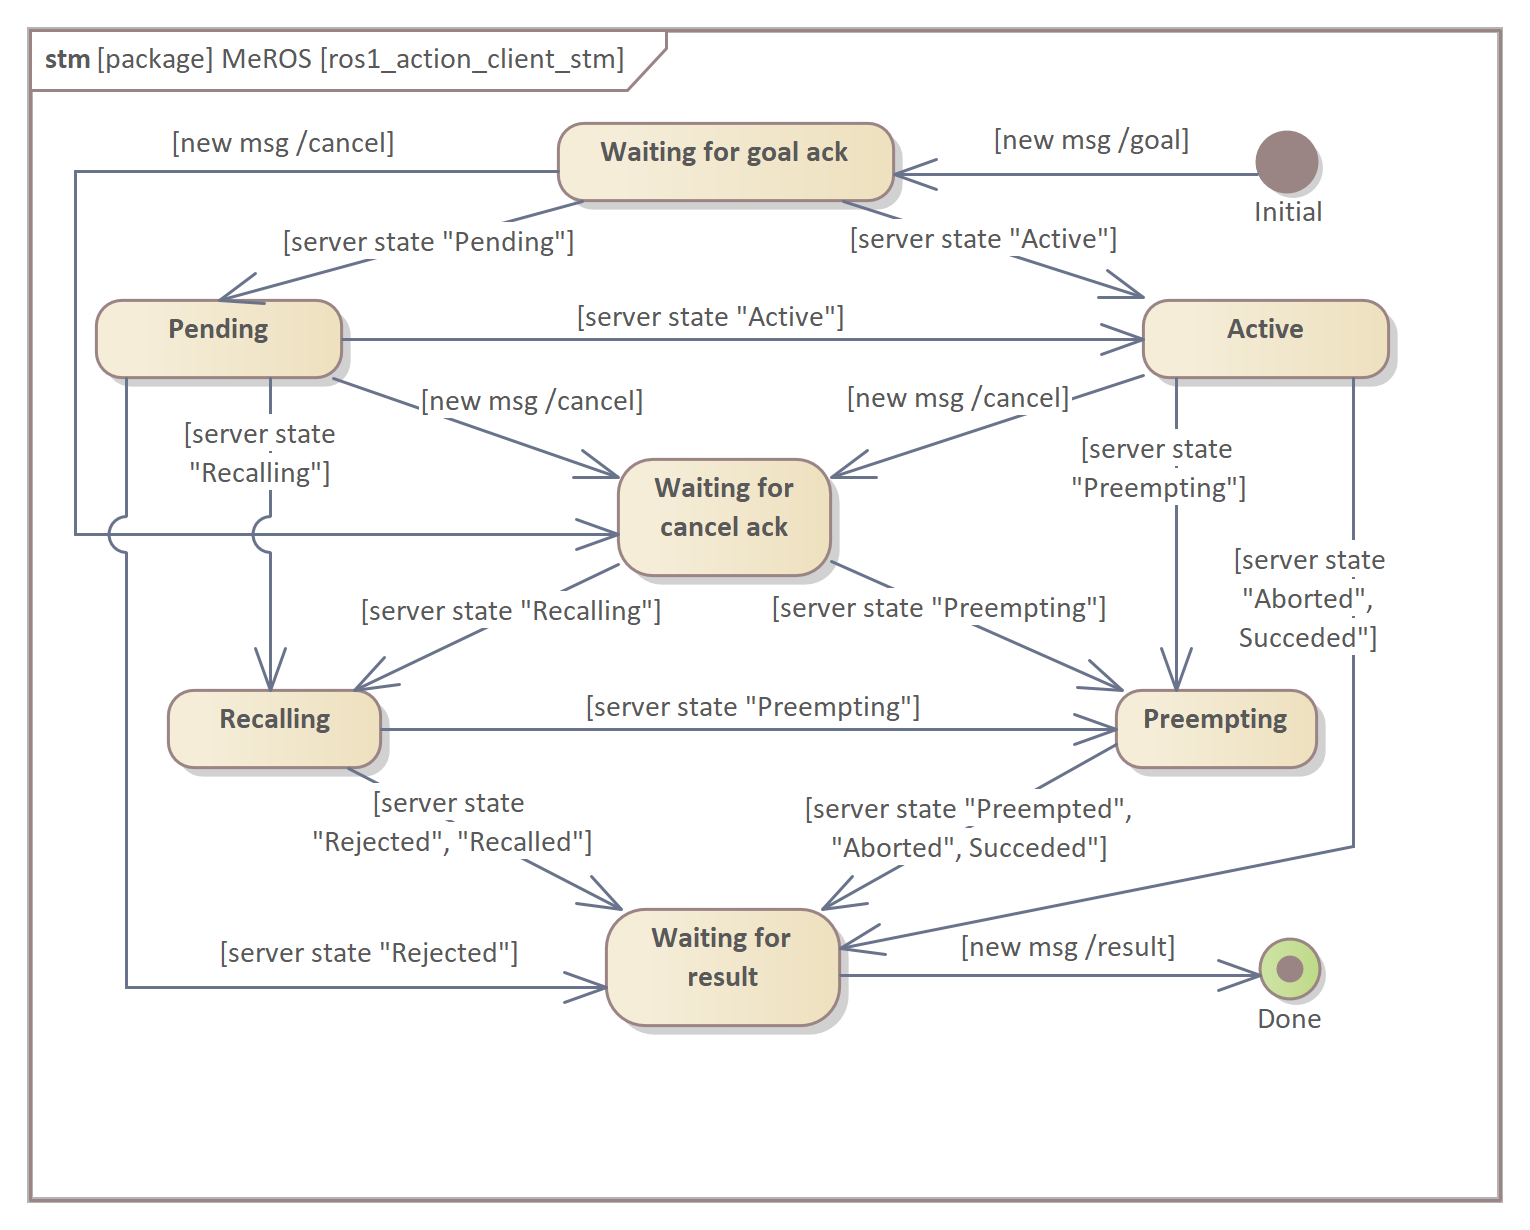
\includegraphics[scale=1.0]{../imgs/meros_pkg/ros1_action_client_stm.png}}
    \end{center}
    \caption{ROS~1 Action client -- stm.}
    \label{fig:ros1_action_client_stm}
\end{figure}
